% !TeX encoding = UTF-8

% 载入 SJTUThesis 模版
\documentclass[type=bachelor, zihao = 5]{sjtuthesis}
% 选项
%   type=[doctor|master|bachelor|course],     % 可选(默认:doctor),论文类型
%   zihao=[-4|5],                             % 可选(研究生默认:-4,本科默认:5),正文字号大小
%   lang=[zh|en],                             % 可选(默认:zh),论文的主要语言
%   review,                                   % 可选(默认:关闭),盲审模式
%   [twoside|oneside]                         % 可选(默认:twoside),单双页模式

% 论文基本配置,加载宏包等全局配置
% !TEX root = ./main.tex

\sjtusetup{
  %
  %******************************
  % 注意:
  %   1. 配置里面不要出现空行
  %   2. 不需要的配置信息可以删除
  %******************************
  %
  % 信息录入
  %
  info = {%
    %
    % 标题
    %
    title           = {波浪场细长体入水过程数值模拟研究},
    title*          = {Numerical simulation study of water entry process of slender body in wave field},
    %
    % 标题页标题
    %   可使用“\\”命令手动控制换行
    %
    % display-title   = {上海交通大学学位论文\\ \LaTeX{} 模板示例文档},
    % display-title*  = {A Sample Document \\ for \LaTeX-based SJTU Thesis Template},
    %
    % 页眉标题
    %
    % running-title   = {示例文档},
    % running-title*  = {Sample Document},
    %
    % 关键词
    %
    keywords        = {入水, 空泡, 波浪场, 数值模拟},
    keywords*       = {water entry, cavity, wave field, CFD},
    %
    % 姓名
    %
    author          = {解煚焱},
    author*         = {Xie Jiongyan},
    %
    % 指导教师
    %
    supervisor      = {陈瑛},
    supervisor*     = {Chen ying},
    %
    % 副指导教师
    %
    % assisupervisor  = {某某教授},
    % assisupervisor* = {Prof. Uom Uom},
    %
    % 学号
    %
    id              = {518021911249},
    %
    % 学位
    %   本科生不需要填写
    %
    degree          = {工学硕士},
    degree*         = {Master of Engineering},
    %
    % 专业
    %
    major           = {工程力学},
    major*          = {engineering mechanics},
    %
    % 所属院系
    %
    department      = {船舶海洋与建筑工程学院},
    department*     = {Depart of Marine, Marine and Architectural Engineering},
    %
    % 课程名称
    %   仅课程论文适用
    %
    course          = {某某课程},
    %
    % 答辩日期
    %   使用 ISO 格式 (yyyy-mm-dd);默认为当前时间
    %
    % date            = {2014-12-17},
    %
    % 资助基金
    %
    % fund  = {
    %           {国家 973 项目 (No. 2025CB000000)},
    %           {国家自然科学基金 (No. 81120250000)},
    %         },
    % fund* = {
    %           {National Basic Research Program of China (Grant No. 2025CB000000)},
    %           {National Natural Science Foundation of China (Grant No. 81120250000)},
    %         },
  },
  %
  % 风格设置
  %
  style = {%
    %
    % 本科论文页眉 logo 颜色 (red/blue/black)
    %
    % header-logo-color = black,
  },
  %
  % 名称设置
  %
  name = {
    % bib               = {References},
    % acknowledgements  = {谢\hspace{\ccwd}辞},
    % publications      = {攻读学位期间完成的论文},
  },
}

% 使用 BibLaTeX 处理参考文献
%   biblatex-gb7714-2015 常用选项
%     gbnamefmt=lowercase     姓名大小写由输入信息确定
%     gbpub=false             禁用出版信息缺失处理
\usepackage[backend=biber,style=gb7714-2015]{biblatex}
% 文献表字体
% \renewcommand{\bibfont}{\zihao{-5}}
% 文献表条目间的间距
\setlength{\bibitemsep}{0pt}
% 导入参考文献数据库
\addbibresource{bibdata/thesis.bib}

% 定义图片文件目录与扩展名
\graphicspath{{figures/}}
\DeclareGraphicsExtensions{.pdf,.eps,.png,.jpg,.jpeg}

% 确定浮动对象的位置,可以使用 [H],强制将浮动对象放到这里(可能效果很差)
% \usepackage{float}

% 固定宽度的表格
% \usepackage{tabularx}

% 使用三线表:toprule,midrule,bottomrule。
\usepackage{booktabs}

% 表格中支持跨行
\usepackage{multirow}

% 表格中数字按小数点对齐
\usepackage{dcolumn}
\newcolumntype{d}[1]{D{.}{.}{#1}}

% 使用长表格
\usepackage{longtable}

% 附带脚注的表格
\usepackage{threeparttable}

% 附带脚注的长表格
\usepackage{threeparttablex}

% 算法环境宏包
\usepackage[ruled,vlined,linesnumbered]{algorithm2e}
% \usepackage{algorithm, algorithmicx, algpseudocode}

% 代码环境宏包
\usepackage{listings}
\lstnewenvironment{codeblock}[1][]%
  {\lstset{style=lstStyleCode,#1}}{}

% 物理科学和技术中使用的数学符号,定义了 \qty 命令,与 siunitx 3.0 有冲突
% \usepackage{physics}

% 直立体数学符号
\newcommand{\dd}{\mathop{}\!\mathrm{d}}
\newcommand{\ee}{\mathrm{e}}
\newcommand{\ii}{\mathrm{i}}
\newcommand{\jj}{\mathrm{j}}

% 国际单位制宏包
\usepackage{siunitx}[=v2]

% 定理环境宏包
\usepackage{ntheorem}
% \usepackage{amsthm}

% 绘图宏包
\usepackage{tikz}
\usetikzlibrary{shapes.geometric, arrows}

% 一些文档中用到的 logo
\usepackage{hologo}
\newcommand{\XeTeX}{\hologo{XeTeX}}
\newcommand{\BibLaTeX}{\textsc{Bib}\LaTeX}

% 借用 ltxdoc 里面的几个命令方便写文档
\DeclareRobustCommand\cs[1]{\texttt{\char`\\#1}}
\providecommand\pkg[1]{{\sffamily#1}}

% 自定义命令

% E-mail
\newcommand{\email}[1]{\href{mailto:#1}{\texttt{#1}}}

% hyperref 宏包在最后调用
\usepackage{hyperref}

% 自动引用题注更正为中文
\def\equationautorefname{式}
\def\footnoteautorefname{脚注}
\def\itemautorefname{项}
\def\figureautorefname{图}
\def\tableautorefname{表}
\def\partautorefname{篇}
\def\appendixautorefname{附录}
\def\chapterautorefname{章}
\def\sectionautorefname{节}
\def\subsectionautorefname{小节}
\def\subsubsectionautorefname{小节}
\def\paragraphautorefname{段落}
\def\subparagraphautorefname{子段落}
\def\FancyVerbLineautorefname{行}
\def\theoremautorefname{定理}


\begin{document}

%TC:ignore

% 标题页
\maketitle

% 原创性声明及使用授权书
\copyrightpage
% 插入外置原创性声明及使用授权书
% \copyrightpage[scans/sample-copyright-old.pdf]

% 前置部分
\frontmatter

% 摘要
% !TEX root = ../main.tex

\begin{abstract}
  入水是指航行体从空气进入水面的过程。在航行体入水时,会携带一部分气体进入水中,或者会使水汽化成水蒸气,这便是入水空泡/空化现象。入水问题是当前科研领域的一个关键问题,研究由来已久。当前阶段,空泡入水是入水问题研究的热点方向。空泡入水问题在波浪场环境下的研究相对不够充分,因此本论文研究了波浪场环境下的空泡入水问题。

  入水空泡这一问题的研究是一个悠久问题,并且一直是流体领域的研究热点和难点。早在 20 世纪初期,入水时受到的冲击就已经有了许多研究,随后至 20 世纪后半页,入水空泡和空化问题逐渐引起了研究的重视。对于入水问题,早期的研究方法包括理论求解,实验验证等,后来逐步开始采用有限元,PIV 或者 CFD 数值模拟的方法。本论文使用的是 CFD 方法对入水空泡问题进行数值模拟。

  航行体进入波浪场时,航行体和波浪场中水和空气的行为都可由物理学和流体力学基础数学模型描述。包括流体的连续性方程,动量方程以及能量守恒方程。之后,又论述了多相流环境下的流体力学基本方程的相关变化。最后又论述了入水空泡模型。这些数学模型是进行数值模拟的基础。

  为了实现数值模拟,本文借助流体力学计算软件 Fluent 进行数值模拟。首先,本文介绍了采用的几何模型和网格划分,其次,给定了各个边的边界条件,并论述了具体的消波方法。为了防止出水区边界造成波浪反射现象,在波浪场中增加一部分消波区,并且在该区域内采用动量源项消波法的方法。为了更好地捕捉界面,采用 VOF 方法进行捕捉。航行体入水过程中,为了让航行体周围的流场情况更加精确,采用重叠网格技术,将包裹航行体的动网格和环境的静态网格可以融合在一起进行流场求算。最后论述了本次实验的具体设置实验设计,根据不同入射角度和入射相位,总计进行了 9 组实验。

  最后,本文对 9 组数值模拟实验进行分析和现象归纳。首先展示了稳定的波浪场结果,其次大致描述了不同入水阶段的密度分布。之后以 $60 ^\circ$ 入水和 $90 ^\circ$ 入水的各一个算例为例,详述了入水过程中的密度场,压力场和速度场。最后分析和论述了各算例下航行体入水过程的特点。
\end{abstract}

\begin{abstract*}
  Water entry refers to the process in which a vehicle enters the water surface from the air. When the vehicle enters the water, it will carry a part of the gas into the water, or it will vaporize the water into water vapor, which is the phenomenon of water entry cavitation/cavitation. The problem of water entry is a key issue in the current scientific research field, and the research has a long history. At the current stage, cavitation into water is a hot research direction of water entry. The research on the problem of cavitation into water in the wave field environment is relatively insufficient, so this paper studies the problem of cavitation into the water in the wave field environment.

  The study of water entry cavitation is a long-standing problem, and has always been a hot and difficult research topic in the field of fluids. As early as the early 20th century, there have been many studies on the impact of water entry, and then to the second half of the 20th century, the problems of water entry cavitation and cavitation gradually attracted research attention. For the water entry problem, the early research methods include theoretical solution, experimental verification, etc., and then gradually began to use finite element, PIV or CFD numerical simulation methods. In this paper, the CFD method is used to numerically simulate the water entry cavitation problem.

  When a vehicle enters the wave field, the behavior of water and air in both the vehicle and the wave field can be described by mathematical models based on physics and fluid mechanics. Including fluid continuity equation, momentum equation and energy conservation equation. Afterwards, the related changes of the basic equations of fluid mechanics in the multiphase flow environment are discussed. Finally, the water entry cavitation model is discussed. These mathematical models are the basis for performing numerical simulations.

  In order to realize the numerical simulation, this paper uses the fluid mechanics calculation software Fluent to carry out the numerical simulation. Firstly, this paper introduces the adopted geometric model and mesh division. Secondly, the boundary conditions of each edge are given, and the specific wave elimination method is discussed. In order to prevent the wave reflection phenomenon caused by the boundary of the water outlet, a part of the wave absorbing area is added to the wave field, and the method of the momentum source term wave absorbing method is used in this area. In order to better capture the interface, the VOF method is used to capture. In the process of entering the water, in order to make the flow field around the vehicle more accurate, the overlapping grid technology is used, and the dynamic mesh surrounding the vehicle and the static mesh of the environment can be integrated to calculate the flow field. Finally, the specific experimental design of this experiment is discussed. According to different incident angles and incident phases, a total of 9 groups of experiments are carried out.

  Finally, this paper analyzes and summarizes the phenomena of 9 groups of numerical simulation experiments. First, the stable wave field results are shown, and second, the density distribution at different water entry stages is roughly described. Then, the density field, pressure field and velocity field in the process of water entry are described in detail by taking one example of $60 ^\circ$ entering water and $90 ^\circ$ entering water as examples. Finally, the characteristics of the water entry process of the vehicle in each case are analyzed and discussed.
\end{abstract*}


% 目录
\tableofcontents
% 插图索引
% \listoffigures*
% 表格索引
% \listoftables*
% 算法索引
% \listofalgorithms*

% 符号对照表
% % !TEX root = ../main.tex

\begin{nomenclature*}
\label{chap:symb}

\begin{longtable}{rl}
  $\epsilon$  & 介电常数  \\  
  $\mu$       & 磁导率    \\
  $\epsilon$  & 介电常数  \\
  $\mu$       & 磁导率    \\
  $\epsilon$  & 介电常数  \\
  $\mu$       & 磁导率    \\
  $\epsilon$  & 介电常数  \\
  $\mu$       & 磁导率    \\
  $\epsilon$  & 介电常数  \\
  $\mu$       & 磁导率    \\
  $\epsilon$  & 介电常数  \\
  $\mu$       & 磁导率    \\
  $\epsilon$  & 介电常数  \\
  $\mu$       & 磁导率    \\
  $\epsilon$  & 介电常数  \\
  $\mu$       & 磁导率    \\
  $\epsilon$  & 介电常数  \\
  $\mu$       & 磁导率    \\
  $\epsilon$  & 介电常数  \\
  $\mu$       & 磁导率    \\
  $\epsilon$  & 介电常数  \\
  $\mu$       & 磁导率    \\
  $\epsilon$  & 介电常数  \\
  $\mu$       & 磁导率    \\
  $\epsilon$  & 介电常数  \\
  $\mu$       & 磁导率    \\
  $\epsilon$  & 介电常数  \\
  $\mu$       & 磁导率    \\
  $\epsilon$  & 介电常数  \\
  $\mu$       & 磁导率    \\
  $\epsilon$  & 介电常数  \\
  $\mu$       & 磁导率    \\
  $\epsilon$  & 介电常数  \\
  $\mu$       & 磁导率    \\
  $\epsilon$  & 介电常数  \\
  $\mu$       & 磁导率    \\
  $\epsilon$  & 介电常数  \\
  $\mu$       & 磁导率    \\
  $\epsilon$  & 介电常数  \\
  $\mu$       & 磁导率    \\
  $\epsilon$  & 介电常数  \\
  $\mu$       & 磁导率    \\
  $\epsilon$  & 介电常数  \\
  $\mu$       & 磁导率    \\
  $\epsilon$  & 介电常数  \\
  $\mu$       & 磁导率    \\
  $\epsilon$  & 介电常数  \\
  $\mu$       & 磁导率    \\
  $\epsilon$  & 介电常数  \\
  $\mu$       & 磁导率    \\
  $\epsilon$  & 介电常数  \\
  $\mu$       & 磁导率    \\
  $\epsilon$  & 介电常数  \\
  $\mu$       & 磁导率    \\
\end{longtable}

\end{nomenclature*}


%TC:endignore

% 主体部分
\mainmatter

% 正文内容
% % !TEX root = ../main.tex

\chapter{简介}

这是 \sjtuthesis 的示例文档,基本上覆盖了模板中所有格式的设置。建议大家在使用模
板之前,除了阅读《\sjtuthesis\ 使用文档》,这个示例文档也最好能看一看。

\section{二级标题}

\subsection{三级标题}

\subsubsection{四级标题}

Lorem ipsum dolor sit amet, consectetur adipiscing elit, sed do eiusmod tempor
incididunt ut labore et dolore magna aliqua. Ut enim ad minim veniam, quis
nostrud exercitation ullamco laboris nisi ut aliquip ex ea commodo consequat.
Duis aute irure dolor in reprehenderit in voluptate velit esse cillum dolore eu
fugiat nulla pariatur. Excepteur sint occaecat cupidatat non proident, sunt in
culpa qui officia deserunt mollit anim id est laborum.

\section{脚注}

Lorem ipsum dolor sit amet, consectetur adipiscing elit, sed do eiusmod tempor
incididunt ut labore et dolore magna aliqua. \footnote{Ut enim ad minim veniam,
quis nostrud exercitation ullamco laboris nisi ut aliquip ex ea commodo
consequat. Duis aute irure dolor in reprehenderit in voluptate velit esse cillum
dolore eu fugiat nulla pariatur.}

\section{字体}


上海交通大学是我国历史最悠久的高等学府之一,是教育部直属、教育部与上海市共建的全
国重点大学,是国家“七五”、“八五”重点建设和“211 工程”、“985 工程”的首批建
设高校。经过 115 年的不懈努力,上海交通大学已经成为一所“综合性、研究型、国际化”
的国内一流、国际知名大学,并正在向世界一流大学稳步迈进。 

{\songti 十九世纪末,甲午战败,民族危难。中国近代著名实业家、教育家盛宣怀和一批
  有识之士秉持“自强首在储才,储才必先兴学”的信念,于 1896 年在上海创办了交通大
  学的前身——南洋公学。建校伊始,学校即坚持“求实学,务实业”的宗旨,以培养“第
  一等人才”为教育目标,精勤进取,笃行不倦,在二十世纪二三十年代已成为国内著名的
  高等学府,被誉为“东方MIT”。抗战时期,广大师生历尽艰难,移转租界,内迁重庆,
  坚持办学,不少学生投笔从戎,浴血沙场。解放前夕,广大师生积极投身民主革命,学校
  被誉为“民主堡垒”。}

{\heiti 新中国成立初期,为配合国家经济建设的需要,学校调整出相当一部分优势专业、
  师资设备,支持国内兄弟院校的发展。五十年代中期,学校又响应国家建设大西北的号
  召,根据国务院决定,部分迁往西安,分为交通大学上海部分和西安部分。1959 年 3月
  两部分同时被列为全国重点大学,7 月经国务院批准分别独立建制,交通大学上海部分启
  用“上海交通大学”校名。历经西迁、两地办学、独立办学等变迁,为构建新中国的高等
  教育体系,促进社会主义建设做出了重要贡献。六七十年代,学校先后归属国防科工委和
  六机部领导,积极投身国防人才培养和国防科研,为“两弹一星”和国防现代化做出了
  巨大贡献。}

{\kaishu 改革开放以来,学校以“敢为天下先”的精神,大胆推进改革:率先组成教授代
  表团访问美国,率先实行校内管理体制改革,率先接受海外友人巨资捐赠等,有力地推动
  了学校的教学科研改革。1984 年,邓小平同志亲切接见了学校领导和师生代表,对学校
  的各项改革给予了充分肯定。在国家和上海市的大力支持下,学校以“上水平、创一流”
  为目标,以学科建设为龙头,先后恢复和兴建了理科、管理学科、生命学科、法学和人文
  学科等。1999 年,上海农学院并入;2005 年,与上海第二医科大学强强合并。至此,学
  校完成了综合性大学的学科布局。近年来,通过国家“985 工程”和“211 工程”的建
  设,学校高层次人才日渐汇聚,科研实力快速提升,实现了向研究型大学的转变。与此同
  时,学校通过与美国密西根大学等世界一流大学的合作办学,实施国际化战略取得重要突
  破。1985 年开始闵行校区建设,历经 20 多年,已基本建设成设施完善,环境优美的现
  代化大学校园,并已完成了办学重心向闵行校区的转移。学校现有徐汇、闵行、法华、七
  宝和重庆南路(卢湾)5 个校区,总占地面积 4840 亩。通过一系列的改革和建设,学校
  的各项办学指标大幅度上升,实现了跨越式发展,整体实力显著增强,为建设世界一流大
  学奠定了坚实的基础。}

{\ifcsname fangsong\endcsname\fangsong\else[无 \cs{fangsong} 字体。]\fi 交通大学
  始终把人才培养作为办学的根本任务。一百多年来,学校为国家和社会培养了 20余万各
  类优秀人才,包括一批杰出的政治家、科学家、社会活动家、实业家、工程技术专家和医
  学专家,如江泽民、陆定一、丁关根、汪道涵、钱学森、吴文俊、徐光宪、张光斗、黄炎
  培、邵力子、李叔同、蔡锷、邹韬奋、陈敏章、王振义、陈竺等。在中国科学院、中国工
  程院院士中,有 200 余位交大校友;在国家 23 位“两弹一星”功臣中,有 6 位交大校
  友;在 18 位国家最高科学技术奖获得者中,有 3 位来自交大。交大创造了中国近现代
  发展史上的诸多“第一”:中国最早的内燃机、最早的电机、最早的中文打字机等;新中国
  第一艘万吨轮、第一艘核潜艇、第一艘气垫船、第一艘水翼艇、自主设计的第一代战斗
  机、第一枚运载火箭、第一颗人造卫星、第一例心脏二尖瓣分离术、第一例成功移植同种
  原位肝手术、第一例成功抢救大面积烧伤病人手术等,都凝聚着交大师生和校友的心血智
  慧。改革开放以来,一批年轻的校友已在世界各地、各行各业崭露头角。}

{\ifcsname lishu\endcsname\lishu\else[无 \cs{lishu} 字体。]\fi 截至 2011 年 12
  月 31 日,学校共有 24 个学院 / 直属系(另有继续教育学院、技术学院和国际教育学
  院),19 个直属单位,12 家附属医院,全日制本科生 16802 人、研究生24495 人(其
  中博士研究生 5059 人);有专任教师 2979 名,其中教授 835 名;中国科学院院士 15
  名,中国工程院院士 20 名,中组部“千人计划”49 名,“长江学者”95 名,国家杰出
  青年基金获得者 80 名,国家重点基础研究发展计划(973 计划)首席科学家 24名,国
  家重大科学研究计划首席科学家 9名,国家基金委创新研究群体 6 个,教育部创新团队
  17 个。}

{\ifcsname youyuan\endcsname\youyuan\else[无 \cs{youyuan} 字体。]\fi 学校现有本
  科专业 68 个,涵盖经济学、法学、文学、理学、工学、农学、医学、管理学和艺术等九
  个学科门类;拥有国家级教学及人才培养基地 7 个,国家级校外实践教育基地 5个,国
  家级实验教学示范中心 5 个,上海市实验教学示范中心 4 个;有国家级教学团队 8个,
  上海市教学团队 15 个;有国家级教学名师 7 人,上海市教学名师 35 人;有国家级精
  品课程 46 门,上海市精品课程 117 门;有国家级双语示范课程 7 门;2001、2005 和
  2009 年,作为第一完成单位,共获得国家级教学成果 37 项、上海市教学成果 157
  项。}

\chapter{研究背景}

\chapter{超空泡入水问题的基本理论}
超空泡入水过程是一个多介质且时变的流体问题,其基本理论可由多相流数学模型和入水空泡模型进行阐述。
\section{多相流数学模型}
在航行体超空泡进入波浪场的环境下,整体环境为气-液-汽三相的波浪场环境,空气与水均满足流体基本的连续性方程,动量方程以及能量守恒方程,
\begin{equation}
  % \frac{\partial \rho}{\partial t} + \frac{\partial}{\partial x_i} \(\rho u_i\) = 0
  \frac {\partial \rho}{\partial t} + \frac {\partial}{\partial x_i} (\rho u_i) = 0
\end{equation}
\begin{equation}
  \frac {\partial (\rho u_i)}{\partial t} + \frac {\partial (\rho u_i u_j)}{\partial x_j} = \frac {\partial}{\partial x_j} \left[ \mu \left( \frac {\partial u_i}{\partial x_j} + \frac {\partial u_j}{\partial x_i} \right) \right] - \frac {\partial}{\partial x_i} \left( p + \frac 2 3 \mu \frac {\partial u_k}{\partial x_k} \right)
\end{equation}
\begin{equation}
  \frac \partial {\partial t} (\rho E) + \frac \partial {\partial x_i} \left( u_i (\rho E + p) \right) = \frac \partial {\partial x_i} \left( k \frac {\partial T}{\partial x_i} \right)
\end{equation}

上式为连续性方程,动量方程以及能量守恒方程的张量表示法,其中$\rho$为流体密度,$\mu$ 为动力学粘性系数,$p$ 为压强,$E$ 为内能与动能之和。$u_i$为流体速度,是一个三维向量。

实际的入水过程都需要借助湍流模型表述\cite{Kliafas1987},对于流场中的气体和液体,均满足
\begin{equation}
  \frac {\partial \rho \phi}{\partial t} + \nabla \cdot (\rho \phi \mathbf u) = \nabla \cdot (\Gamma \nabla \phi) + S_{\phi}
\end{equation}
其中 $\phi$ 是流场中关于 $\mathbf x$ 和 $t$ 的连续函数。

在气液两相流的环境下,需要引入各相的体积分数,满足,
\begin{equation}
  \sum _{q = 1} ^3 \alpha _q = 1
\end{equation}
由于两相流模型中气液均满足相同形式的控制方程,因而混合介质下的各物理量可表达为以下形式:
\begin{equation}
  \phi = \begin{cases}
    \sum _{q = 1} ^3 \alpha_q \phi_q & \phi = \rho, \mu \\
    \sum _{q = 1} ^3 \alpha_q \phi_q \rho_q \bigg/ \sum _{q = 1} ^3 \alpha _q \rho _q & \phi = E, T
  \end{cases}
\end{equation}
而各相还需要满足输运方程:
\begin{equation}
  \frac {\partial (\rho _q \alpha _q)} {\partial t} + \frac {\partial (\rho _q \alpha _q u_i)}{\partial t} = \begin{cases}
    0 & q = gas \\
    S & q = vapor
  \end{cases}
  \label{eq:transport}
\end{equation}

\section{入水空泡模型}

\subsection{自由面空气和气体空泡模型}
本项目的入水问题采用 Mixture 模型,对于航行体入水时形成的空泡,其中气相体积也满足方程\ref{eq:transport},故有,
\begin{equation}
  \frac \partial {\partial t} (\rho _g \alpha_g) + \frac \partial {\partial x_i} (\rho _g \alpha _g u_i) = 0
\end{equation}

\subsection{空化模型}
当物体超高速($10^3 m/s$)入水时,会发生显著的自然空化现象,其中蒸汽相满足以下形式的输运方程:
\begin{equation}
  \frac {\partial \alpha _v}{\partial t} + \frac \partial {\partial x_j} (u_j a_v) = S_e - S_c
\end{equation}
其中 $S_e - S_c$ 为相变速率,典型的空化模型中,有,
\begin{equation}
  S_e = C_e \rho _v \alpha _l \frac {\max (p_v - p, 0)} {(1 / 2 p_l U _{\infty} ^2) t _{\infty}}
\end{equation}
\begin{equation}
  S_c = C_c \frac {\rho _v}{t _{\infty}} (\alpha _l - \alpha _g) ^2 (1 - \alpha_l 0 \alpha_g)
\end{equation}
其中 $C$ 为经验系数,下标 $l$、$v$、$g$ 分别代表液相、蒸汽相和气相,$\alpha$ 为各相的体积分数。
\chapter{数值计算方法}
为了实现对超空泡物体进入波浪场的模拟,本文借助流体力学计算软件 Fluent 对不同的入水条件进行数值模拟。本文首先确定了计算的几何模型和区域,进行恰当的网格划分,给予合适的 UDF 边界条件,选用适当的数值方法,从而实现了波浪场的模拟。之后借助界面捕捉的 VOF 方法以及重叠网格技术,实现了航行体入水的方案设计。
\section{几何模型和网格划分}
本文为了模拟五级海况\cite{Xia1987}的环境,选取的环境场背景网格为 $300 \mathrm m \times 60 \mathrm m \times 10 \mathrm m$ 的长方体区域。模拟水深 $40 \mathrm m$,波长 $40 \mathrm m$,波高近 $3 \mathrm m$。由于水面附近的计算精度要求高,故以水面所在平面为最精细的网格,两侧以一定比例按等比数列扩大其网格间距。入水过程发生在波浪船舶方向的 $0 < x < 200$ 范围内,后半区域 $200 < x < 300$ 为消波区。工作区划分为均匀网格,每个波长内大约80个网格,消波区采用快速增大的粗糙网格,总体网格量为84万,可以足够精细地描述波浪场环境。

运动网格为围绕入水细长航行体的圆柱体网格。细长航行体的长度$5 \mathrm m$,直径$0.5 \mathrm m$。网格沿圆柱体轴线方向采用等距划分,沿径向方向从外至内按照等比数列距离缩小,以增强靠近物体表面部分的精度。在模拟过程中,动网格始终环绕着入水物体,与入水物体之间的相对位置保持不变,并使用重叠网格技术以进行区域内的数值模拟。在初始状态下,背景网格与运动网格如图~\ref{fig:overlay_grid}所示

\begin{figure}[!htp]
  \centering
  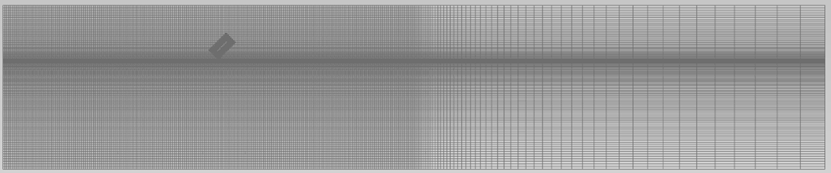
\includegraphics[]{overlay_grid.png}
  \caption[]{入水角度 $45 ^ \circ$ 的初始重叠网格}
  \label{fig:overlay_grid}
\end{figure}

\section{边界条件}
采用速度边界作为输入的造波方法进行二阶 Stokes 波的模拟,入口处实时给定波高$\eta$以及 $x$ 方向和 $y$ 方向的水质点速度($u$、$v$)\cite{Zou2005}。
\begin{equation}
  \eta = \frac H 2 \cos (kx - \omega t + \Phi _0) + \frac {k H^2 \cosh k y} {16 \sinh ^3 kd} (\cosh 2kd + 2)cos2(kx - \omega t)
\end{equation}
\begin{equation}
  u = \frac {\pi H} T \frac {\cosh k(y + d)} {sinh kd} \cos (kx - \omega t) + \frac 3 4 \frac {\pi H} T \left( \frac {\pi H} L \right) \frac {\cosh 2k(y + d)} {\sinh^4 kd} \cos 2(kx - \omega t)
\end{equation}
\begin{equation}
  v = \frac {\pi H} T \frac {\sinh k(y + d)} {sinh kd} + \frac 3 4 \frac {\pi H} T \left( \frac {\pi H} L \right) \frac {\sinh 2k(y + d)} {\sinh^4 kd} \sin 2(kx - \omega t)
\end{equation}

在确定了左侧入口处的速度边界条件后,为了保证入口和出口流量守恒,右侧出口给定与入口 Stokes 波的静漂移相对应的均匀速度。本模型模拟的是三维环境,但 z 方向的动力学特性是轴对称的,因而 z 方向的两个表面采用的是对称面边界条件。$y = 0$ 的边界为海底,给定固壁边界条件,$y = 60$ 的边界为大气,给定压力出口边界。

\section{动量源项消波法}
单纯采用速度边界作为输入时,会发生波浪反射的现象,影响波浪场效果。对于这个问题,可以采用动量源项消波法使结果更准确\cite{Wang2005,Li2013,Peric2015}。本文使用动量源项消波法的区域为 $200 < x < 300$ 的消波区。对于 Navier-Stokes 方程,增加一动量源项,有
\begin{equation}
  \frac {\partial (\rho u_i)}{\partial t} + \frac {\partial (\rho u_i u_j)}{\partial x_j} = \frac {\partial}{\partial x_j} \left[ \mu \left( \frac {\partial u_i}{\partial x_j} + \frac {\partial u_j}{\partial x_i} \right) \right] - \frac {\partial}{\partial x_i} \left( p + \frac 2 3 \mu \frac {\partial u_k}{\partial x_k} \right) + S_i
\end{equation}
其中 $\mathbf S$ 即为增加的动量源项,可采用如下形式确定:
\begin{equation}
  S_i = [C(x) - 1]\left[ \frac \rho {\Delta t} (u_{iC} - U_i) - \rho u_{jC} \frac {\partial u_{iC}}{\partial x_j} - \frac {\partial p_c} {\partial x_i} + \rho f_i \right]
\end{equation}
其中 $C(x)$ 为任意光滑函数,下标 $C$ 为计算值。在本次模拟场景下,C(x)取值为
\begin{equation}
  C(x) = 0.9985 + 0.0015 t - 0.9985 e^{-t/0.025}, t = 1 - \frac x l
\end{equation}
其中 $x$ 为质点距消波区左端的距离, $l$ 为消波区长度

\section{数值方法}
数值模拟在上述网格划分和边界条件等的基础之上,借助商业计算流体软件 Fluent,设定具体地数值方法。模型整体是基于压力的时变迭代方法,考虑重力的影响。以水为主相,气为次相,水相为不可压缩流体,气相采用理想气体模型考虑其压缩性。采用RNG k-epsilon模型结合壁面函数的方法计算湍流效应。数值算法采用压力速度耦合算法。

\section{界面捕捉的 VOF 方法}
在通常的数值模拟过程中,我们在每个单元中对每相使用一个值 $\alpha$ 来表示该相的体积分数,并确保各项的体积分数之和为 $1$,但这种表示方法没有给出各项在这个单元内的交界面形状,使用 VOF 方法则可以重构出交界面形状\cite{HIRT1981},例如,使用平行于网格的直线对交界面进行拟合,对应的则为 SOLA-VOF 算法。本模拟过程采用的是二阶 PLIC 算法,可以得到更精确的自由面和空泡形状。这种 VOF 界面捕捉方法与前述的动量源项消波法完全兼容\cite{Li2013}。

\section{重叠网格技术}

% --- 这块是复制粘贴的

我们将航行体包裹在一小块子区域中,该子区域处于整个计算区域工作区的适当位置。针对子区域和外部计算域的不同疏密要求分别划分网格。子区域与外部区域的交界处通过滑移面相互匹配,并使网格尽量均匀过渡。
由于入水问题的计算域是随时间变化的,我们将采用动网格技术实现不断变化的求解域。动网格的方法根据每个时刻边界的新位置对网格进行自动更新。存在移动边界的任意控制体上的某一标量 $\phi$ 的守恒方程的积分形式可以写作:

\begin{equation}
  \int _V \frac {\partial (\rho \phi)} {\partial t} \mathrm dV + \int_A \rho \phi (u_i - (u_g)_i) \mathrm d A_i = \int_V S_\phi \mathrm dV + \int _A \Gamma \frac {\partial \phi}{\partial x_i} \mathrm d A_i
\end{equation}
其中 $u_g$ 是网格移动速度。

边界的运动导致计算域的网格也要发生相应的运动和变形。动网格方法中,有一类区域的网格只发生一定的运动,构成单元的各个面的运动速度相同,因此网格本身并没有变形。此时,只要采用如上式的控制方程即可,而不必额外对网格进行调整。另一类区域的网格必须通过变形才能调整,它根据当前时刻的边界位置和速度以及时间步长,确定下一时刻的边界位置,再在邻近移动边界的局部区域对网格进行调整,甚至重新划分网格。弹簧平滑方法、动态分层方法、网格重构等方法都是较为常用的方法。针对航行体出水问题的特点,我们在计算过程中将尽量采用动态分层方法,通过滑移面使包裹着航行体的子区域相对于外部区域向上运动。

在结构化网格中,所有与移动区域相邻的网格拓扑结构都是柱形,可以使用动态铺层方法。它根据动边界附近层的高度来添加或移除与移动边界相邻的网格层。

动态铺层法指定在每一个动边界附近的理想层高度。根据网格层$j$的高度,相邻于动边界的网格层$j$被分割或者与附近的网格层$i$合并。如果$j$层上的网格拉伸了,网格高度可以扩展到:

\begin{equation}
  h_{\min} > (1 + \alpha _s) h_{\mathrm{ideal}}
\end{equation}

式中, $h_{\min}$ 是$j$层网格的最小高度,$h_{\mathrm{ideal}}$ 是理想网格高度, $\alpha _s$是分裂因子。当达到上述条件后,网格将根据指定的固定高度或者固定比率进行分割。当指定固定高度时,网格层会分裂成两层,一层是固定高度$h_{\mathrm{ideal}}$,另一层是$h - h_{\mathrm{ideal}}$ ;当指定固定比率时,新生成的网格高度比率为 $\alpha_s$,如果$j$层上的网格被压缩时,压缩将进行到下式的程度:
\begin{equation}
  h_{\min} < \alpha _c h_{\mathrm {ideal}}
\end{equation}
式中, $\alpha _c$是溃灭因子。当达到上面的条件时,被压缩的层$j$就会和它之上的层$i$合并。

对于非结构化网格,采用局部网格重构法更新网格。
局部网格重构法将那些不满足倾斜度或者大小准则的网格标记,然后重新生成网格,同时将计算得到的变量值插值到旧网格上:(a)网格大于指定的最大网格尺寸。(b)网格小于指定的最小网格尺寸。(c)网格倾斜度大于指定的最大倾斜度。
以简单的四面体网格构成的圆柱为例。当其底部移动时,采用与动态铺层法类似的方法,分析连接在边界上的网格高度,根据指定的理想面高和分离/合并因子来分离或合并网格。当第$j$层网格拉伸时,如果$h_{\min} > (1 + \alpha_h) h_{\mathrm{ideal}}$,网格面就根据预先设定的面高分裂,新的面高等于理想面高。当第$j$层压缩时,如果满足$h_{\min} < \alpha _h h_{\mathrm{ideal}}$,被压缩的层$j$则与之上的层$i$合并。这里的$h_{\mathrm{ideal}}$是理想面高,$\alpha$是高度因子。

\section{实验设计}

为了探究不同入射角度和入射相位对航行体运动的影响,在方案设计中会针对不同入射角度和入射相位进行数值模拟实验。在对航行体入水过程进行模拟之前,首先使航行体在水面上方以一定的姿态保持静止状态,以选取的波浪参数进行数值水池造波。然后,待工作区的波面形状趋于稳定状态之后,采用重叠网格方法和动网格技术使航行体的网格子区域开始向下(垂直或带倾角)运动。根据所需要的入水波浪相位,调整好恰当的航行体启动时刻,以指定的入水速度和入水角度运动至水面,之后的入水阶段采用完全自由运动。

针对航行体在不同波浪相位($0 ^\circ$ - $270 ^\circ$)入水过程进行数值模拟时,$0^\circ$相位表示航行体头部触及水面时位于波浪的波峰位置,$180^\circ$相位表示位于波谷位置,$90^\circ$和$270^\circ$相位表示位于波峰和波谷的中间位置。

对于不同的波浪相位和航行体倾角,航行体在启动时刻之后的初始运动速度均统一为 $10 m/s$,运动总时长 $t$ 为 $2s$,每个时间步为 $0.001s$,每个时间步迭代 50 次。
\chapter{数值模拟结果与分析}
本次实验共运行了 9 个样例,航行体入水角度分别为 $90 ^\circ$ 垂直入水以及 $60 ^\circ$ 和$45 ^\circ$入水。所有样例的均运行 2 秒,并保留了各运行时段的动力学状态。

\section{稳定的波浪场结果}
在进行完网格划分,边界条件设计,引入动量源项消波法之后,通过合适的数值方法,成功模拟了稳定的波浪场结果。下面为波浪传播某时刻的密度图,压强分布图和速度分布图。本文的算例是三维算例,但为了更直观地展示计算的结果,选取了在 $z$ 方向为对称轴的剖面进行图形的绘制。如无特殊说明,本文中展示的二维流场图形(如密度图,流场速度图等)均为在 $z$ 方向对称轴位置的流场结果。

\begin{figure}[!htp]
  \centering
  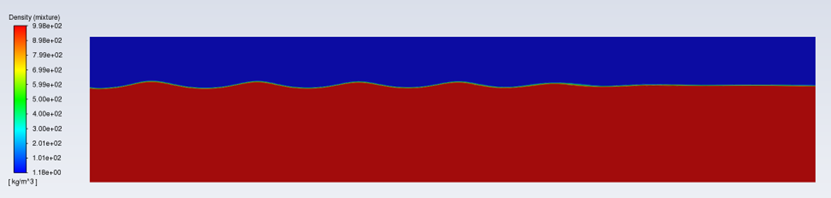
\includegraphics[]{fig/wave_density.png}
  \caption{波浪场密度($\rho$)图}
\end{figure}

波浪场压强分布如图\ref{fig:wave_pressure}所示,可以看到,空气和水体之间的压力区分明显,液体区域随深度增加压强逐渐升高。
\begin{figure}[!htp]
  \centering
  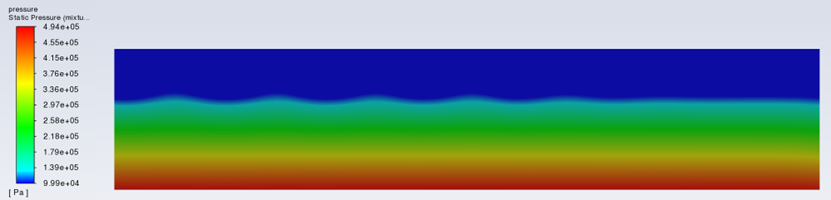
\includegraphics[]{fig/wave_pressure.png}
  \caption{波浪场压强($p$)分布图}
  \label{fig:wave_pressure}
\end{figure}

波浪场速度分布图如图\ref{fig:wave_u},\ref{fig:wave_v}所示,在工作区呈现典型的波浪场速度分布特征,在消波区存在一定的$u$分布,也符合动量源项消波法的结果。
\begin{figure}[!htp]
  \centering
  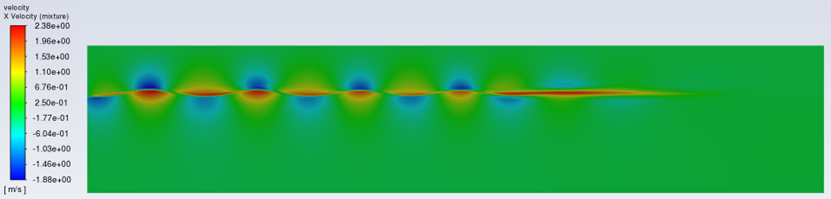
\includegraphics[]{fig/wave_u.png}
  \caption{波浪场$x$方向速度($u$)分布图}
  \label{fig:wave_u}
\end{figure}
\begin{figure}[!htp]
  \centering
  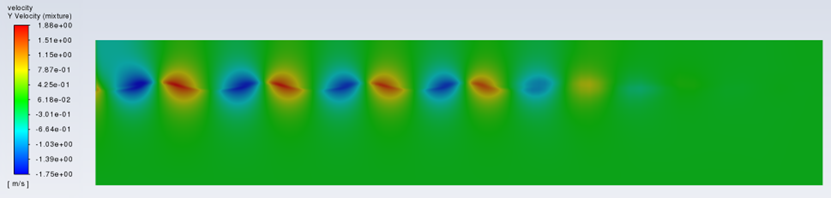
\includegraphics[]{fig/wave_v.png}
  \caption{波浪场$y$方向速度($v$)分布图}
  \label{fig:wave_v}
\end{figure}

\section{不同入水阶段的密度分布}
在考虑并应用 VOF 捕捉方法和重叠网格技术后,可以顺利地进行入水数值模拟实验。数值模拟实验共进行 $t_{\max} = 2s$。以下是入射倾角为 $45^\circ$ 时,运行 $0s$、$0.5$、$0.7s$、$0.9s$、$2.0s$ 的局部密度图。

\begin{figure}[!htp]
  \centering
  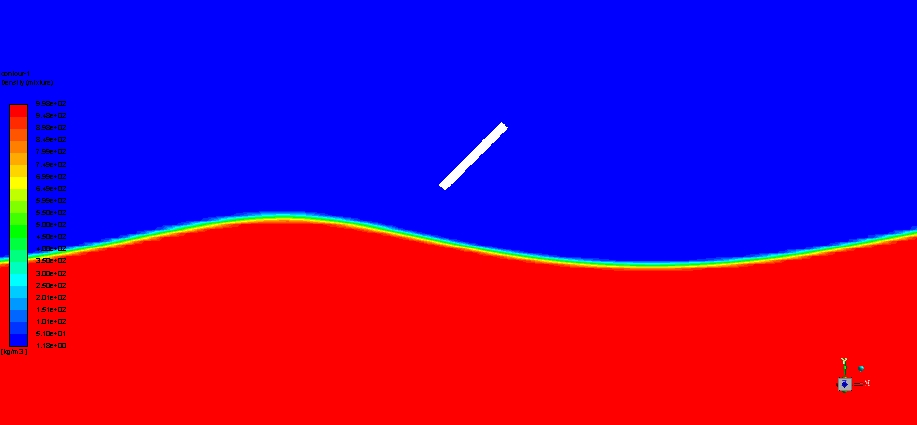
\includegraphics[width=0.5\textwidth]{fig/WaterEntry-AOA45-1-0.jpg}
  \caption{$t=0s$时局部密度图} 
\end{figure}

\begin{figure}[!htp]
  \centering
  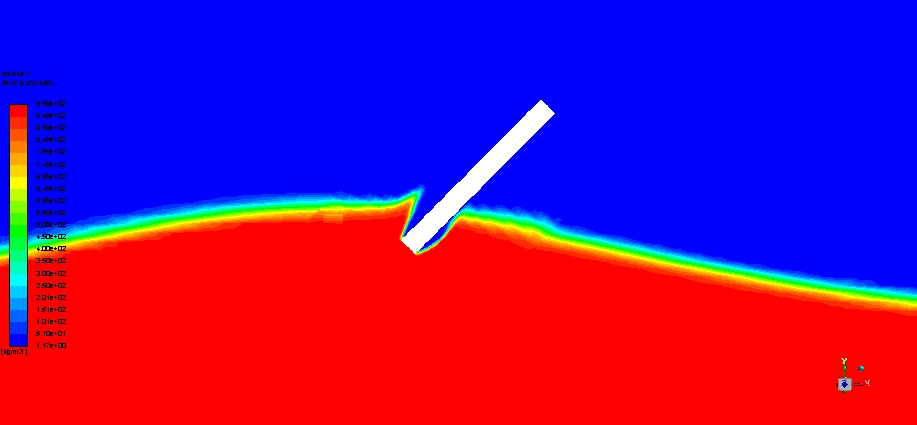
\includegraphics[width=0.5\textwidth]{fig/WaterEntry-AOA45-1-0_5.jpg}
  \caption{$t=0.5s$时局部密度图}
\end{figure}

\begin{figure}[!htp]
  \centering
  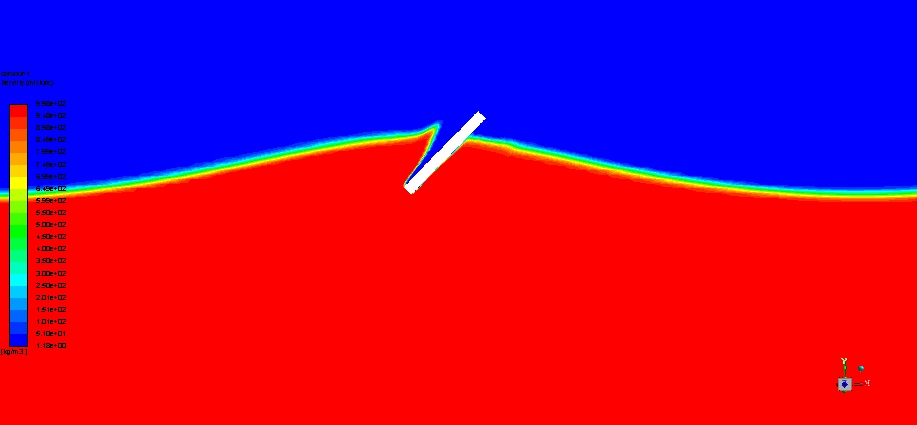
\includegraphics[width=0.5\textwidth]{fig/WaterEntry-AOA45-1-0_7.jpg}
  \caption*{$t=0.7s$时局部密度图} 
\end{figure}

\begin{figure}[!htp]
  \centering
  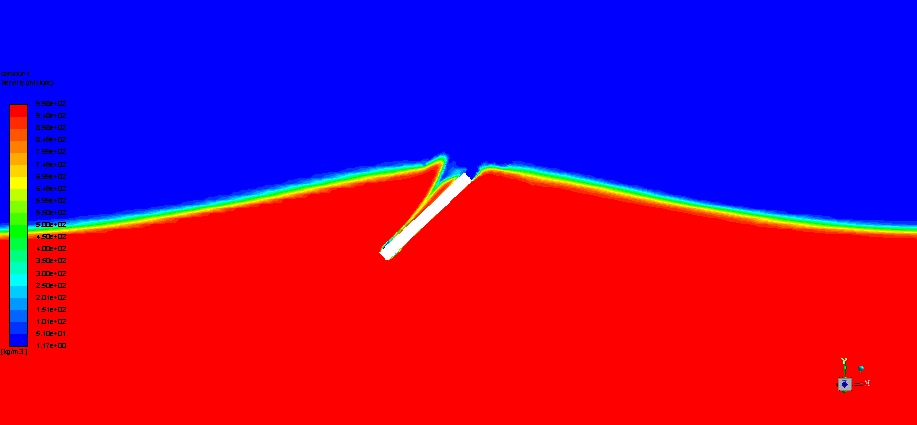
\includegraphics[width=0.5\textwidth]{fig/WaterEntry-AOA45-1-0_9.jpg}
  \caption{$t=0.9s$时局部密度图} 
\end{figure}

\begin{figure}[!htp]
  \centering
  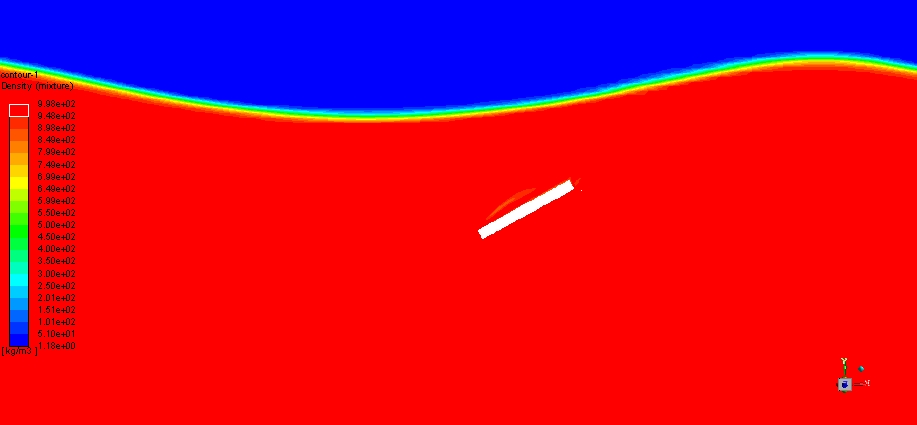
\includegraphics[width=0.5\textwidth]{fig/WaterEntry-AOA45-1-2_000000.jpg}
  \caption{$t=2.0s$时局部密度图} 
\end{figure}

可以看到入水过程发生了显著的空泡现象。将这些结果与理论分析和实验的结果进行对比,发现与实际符合良好,这也验证了模型的准确性。

\section{入水过程的流场状态细节分析}

为了更好地观察和描述入水过程中的现象,本文首先对入射角度与水面夹角为 $60^\circ$,$90 ^\circ$ 和 $45 ^\circ$ 的各一个算例(均为各入水角度的算例 3 )的入水过程的详细情况进行了分析,从而得到航行体进入波浪场时的一般情况。

\subsection{$60 ^\circ$入水条件下的入水过程流场状态细节}

本文首先对 $60 ^\circ$ 的算例进行了分析,如图\ref{fig:detail_d}所示。可以看到,从 $t = 0.3 s$航行体首次接触波浪场水面开始,大约总共进行了 $0.5 s$ 才使整个航行体全部没入波浪场中。航行体在进入波浪场中的同时,波浪场也在进行运动,在 $t= 0.3s$时,航行体与波浪场的接触点约在相位 $\varphi = \pi$ 左右,而当 $t = 0.8s$ 航行体全部进入水中时,前述位置下波浪场已经运行至 $\varphi = \pi / 2$ 的相位。在 $0.5s$ 的过程中,波浪场运行相位约为 $\pi / 2$,这也与实验中预先给定的 Stokes 波的参数相符合。入水过程中有非常明显的空泡现象。在航行体刚进入水面时,空泡出现在航行体的四周,且从头部至水面都有空泡。随着航行体的不断运行,右下侧的空泡逐渐坍缩,且航行体头部附近的空泡逐渐消失,空泡聚集在了航行体的尾部。在整个航行体运行期间,尽管航行体进入水下并引起了空泡已经扰动,但明显可以发现整个流场还保持非常稳定的波浪场状态。这得益于流场区域在 $z$ 轴方向具有比较大的深度,直径仅为 $0.5m$ 的航行体不会对具有持续波浪的流场产生使整体改变波浪状态的影响。

\begin{figure}[!htp]
  \centering

  \begin{subfigure}{0.25\textwidth}
    \centering
    \includegraphics[width = \textwidth]{fig/aoa60_60st/3d.jpg}
    \caption{$t = 0.3s$}
  \end{subfigure}
  \hspace{1cm}
  \begin{subfigure}{0.25\textwidth}
    \centering
    \includegraphics[width = \textwidth]{fig/aoa60_60st/4d.jpg}
    \caption{$t = 0.4s$}
  \end{subfigure}
  \hspace{1cm}
  \begin{subfigure}{0.25\textwidth}
    \centering
    \includegraphics[width = \textwidth]{fig/aoa60_60st/5d.jpg}
    \caption{$t = 0.5s$}
  \end{subfigure}

  \quad

  \begin{subfigure}{0.25\textwidth}
    \centering
    \includegraphics[width = \textwidth]{fig/aoa60_60st/6d.jpg}
    \caption{$t = 0.6s$}
  \end{subfigure}
  \hspace{1cm}
  \begin{subfigure}{0.25\textwidth}
    \centering
    \includegraphics[width = \textwidth]{fig/aoa60_60st/7d.jpg}
    \caption{$t = 0.7s$}
  \end{subfigure}
  \hspace{1cm}
  \begin{subfigure}{0.25\textwidth}
    \centering
    \includegraphics[width = \textwidth]{fig/aoa60_60st/8d.jpg}
    \caption{$t = 0.8s$}
  \end{subfigure}

  \quad 

  \begin{subfigure}{0.25\textwidth}
    \centering
    \includegraphics[width = \textwidth]{fig/aoa60_60st/12d.jpg}
    \caption{$t = 1.2s$}
  \end{subfigure}
  \hspace{1cm}
  \begin{subfigure}{0.25\textwidth}
    \centering
    \includegraphics[width = \textwidth]{fig/aoa60_60st/16d.jpg}
    \caption{$t = 1.6s$}
  \end{subfigure}
  \hspace{1cm}
  \begin{subfigure}{0.25\textwidth}
    \centering
    \includegraphics[width = \textwidth]{fig/aoa60_60st/20d.jpg}
    \caption{$t = 2.0s$}
  \end{subfigure}

  \caption{$60^\circ$入水角度下第三个算例的密度场}
  \label{fig:detail_d}
\end{figure}

航行过程中的压力图如图\ref{fig:detail_p}所示,图b)至图f)的压力范围均取自 $0.8 \times 10^5 \sim 2 \times 10^5 \mathrm{Pa}$,而图a)的压力范围为$0.8 \times 10^5 \sim 4 \times 10^5 \mathrm{Pa}$,所以会使图a)的背景场看起来与其他场不同。使用不同的压力范围取值是因为图a)接触前端的压力很大。可以看到背景波浪场中,空气部分由于连接大气,其压强保持在 $10^5 \mathrm{Pa}$ 左右,而水内部则随着深度的增加压力逐渐增加。本次数值实验采用的航行体为圆柱体,可以明显看到其前端受到的阻力很大。前端压力最大的情况出现在刚接触水面的时候,在本算例中到达了接近 $4 \times 10^5 \mathrm{Pa}$ 的压力。前端压力在物体刚接触到水面时迅速提升并达到最大值,在航行体前端已经浸入水面后,其前端压力依旧较高,且前端一定区域内都受高压影响,但相对于刚接触水面时保持相对较少水平,且在航行过程中没有太大变化。航行体两侧存在一定的低压区,低压区发生在存在空泡的区域,在 $t = 0.4s$ 和 $t = 0.5s$ 空泡时非常明显,这与空泡现象的理论分析和常规实验结果相一致。航行体前端的侧面是航行体压力最低的区域。在 $t= 0.6s$ 和 $t = 0.7s$ 时航行体右侧空泡已接近消失,右侧局部压力不降反升。

\begin{figure}[!htp]
  \centering

  \begin{subfigure}{0.25\textwidth}
    \centering
    \includegraphics[width = \textwidth]{fig/aoa60_60st/3p.jpg}
    \caption{$t = 0.3s$}
  \end{subfigure}
  \hspace{1cm}
  \begin{subfigure}{0.25\textwidth}
    \centering
    \includegraphics[width = \textwidth]{fig/aoa60_60st/4p.jpg}
    \caption{$t = 0.4s$}
  \end{subfigure}
  \hspace{1cm}
  \begin{subfigure}{0.25\textwidth}
    \centering
    \includegraphics[width = \textwidth]{fig/aoa60_60st/5p.jpg}
    \caption{$t = 0.5s$}
  \end{subfigure}

  \quad

  \begin{subfigure}{0.25\textwidth}
    \centering
    \includegraphics[width = \textwidth]{fig/aoa60_60st/6p.jpg}
    \caption{$t = 0.6s$}
  \end{subfigure}
  \hspace{1cm}
  \begin{subfigure}{0.25\textwidth}
    \centering
    \includegraphics[width = \textwidth]{fig/aoa60_60st/7p.jpg}
    \caption{$t = 0.7s$}
  \end{subfigure}
  \hspace{1cm}
  \begin{subfigure}{0.25\textwidth}
    \centering
    \includegraphics[width = \textwidth]{fig/aoa60_60st/8p.jpg}
    \caption{$t = 0.8s$}
  \end{subfigure}

  \quad 

  \begin{subfigure}{0.25\textwidth}
    \centering
    \includegraphics[width = \textwidth]{fig/aoa60_60st/12p.jpg}
    \caption{$t = 1.2s$}
  \end{subfigure}
  \hspace{1cm}
  \begin{subfigure}{0.25\textwidth}
    \centering
    \includegraphics[width = \textwidth]{fig/aoa60_60st/16p.jpg}
    \caption{$t = 1.6s$}
  \end{subfigure}
  \hspace{1cm}
  \begin{subfigure}{0.25\textwidth}
    \centering
    \includegraphics[width = \textwidth]{fig/aoa60_60st/20p.jpg}
    \caption{$t = 2.0s$}
  \end{subfigure}

  \caption{$60^\circ$入水角度下第三个算例的压力场}
  \label{fig:detail_p}
\end{figure}

航行过程中的水平方向速度$u$图和垂直方向速度 $v$ 图如图\ref{fig:detail_u}和图\ref{fig:detail_v}所示。这些图的坐标刻度都不相同。通过比较各流场时刻的速度分布,可以发现整个背景场的速度分布与二阶 Stokes 波的速度分布符合地很好。尽管受本身时变的波浪背景场的影响,但航行体附近的流场速度场依旧有许多规律,并且与一般的流体力学理论相符合。航行体与接触的流体之间形成固壁边界条件,其前端和尾端都是圆截面,在航行过程中受到较大的阻力。其前端前方和尾端后方的速度场都是与航行体的运行速度方向相一致的。在航行体附近的空泡区域,其运动速度比较大,且速度方向平行于航行体边缘的方向。在 $t = 0.4s$ 和 $t = 0.5s$ 的时刻在航行体的前端空泡处具有逆时针方向的速度。在 $t = 0.6 \sim 0.8 s$ 时,航行体右后方的空泡转移并消失,空泡转移至航行体左上侧,流场运动方向与航行体运动方向相反。 


\begin{figure}[!htp]
  \centering

  \begin{subfigure}{0.25\textwidth}
    \centering
    \includegraphics[width = \textwidth]{fig/aoa60_60st/3u.jpg}
    \caption{$t = 0.3s$}
  \end{subfigure}
  \hspace{1cm}
  \begin{subfigure}{0.25\textwidth}
    \centering
    \includegraphics[width = \textwidth]{fig/aoa60_60st/4u.jpg}
    \caption{$t = 0.4s$}
  \end{subfigure}
  \hspace{1cm}
  \begin{subfigure}{0.25\textwidth}
    \centering
    \includegraphics[width = \textwidth]{fig/aoa60_60st/5u.jpg}
    \caption{$t = 0.5s$}
  \end{subfigure}

  \quad

  \begin{subfigure}{0.25\textwidth}
    \centering
    \includegraphics[width = \textwidth]{fig/aoa60_60st/6u.jpg}
    \caption{$t = 0.6s$}
  \end{subfigure}
  \hspace{1cm}
  \begin{subfigure}{0.25\textwidth}
    \centering
    \includegraphics[width = \textwidth]{fig/aoa60_60st/7u.jpg}
    \caption{$t = 0.7s$}
  \end{subfigure}
  \hspace{1cm}
  \begin{subfigure}{0.25\textwidth}
    \centering
    \includegraphics[width = \textwidth]{fig/aoa60_60st/8u.jpg}
    \caption{$t = 0.8s$}
  \end{subfigure}

  \quad 

  \begin{subfigure}{0.25\textwidth}
    \centering
    \includegraphics[width = \textwidth]{fig/aoa60_60st/12u.jpg}
    \caption{$t = 1.2s$}
  \end{subfigure}
  \hspace{1cm}
  \begin{subfigure}{0.25\textwidth}
    \centering
    \includegraphics[width = \textwidth]{fig/aoa60_60st/16u.jpg}
    \caption{$t = 1.6s$}
  \end{subfigure}
  \hspace{1cm}
  \begin{subfigure}{0.25\textwidth}
    \centering
    \includegraphics[width = \textwidth]{fig/aoa60_60st/20u.jpg}
    \caption{$t = 2.0s$}
  \end{subfigure}

  \caption{$60^\circ$入水角度下第三个算例的水平速度场}
  \label{fig:detail_u}
\end{figure}
\begin{figure}[!htp]
  \centering

  \begin{subfigure}{0.25\textwidth}
    \centering
    \includegraphics[width = \textwidth]{fig/aoa60_60st/3v.jpg}
    \caption{$t = 0.3s$}
  \end{subfigure}
  \hspace{1cm}
  \begin{subfigure}{0.25\textwidth}
    \centering
    \includegraphics[width = \textwidth]{fig/aoa60_60st/4v.jpg}
    \caption{$t = 0.4s$}
  \end{subfigure}
  \hspace{1cm}
  \begin{subfigure}{0.25\textwidth}
    \centering
    \includegraphics[width = \textwidth]{fig/aoa60_60st/5v.jpg}
    \caption{$t = 0.5s$}
  \end{subfigure}

  \quad

  \begin{subfigure}{0.25\textwidth}
    \centering
    \includegraphics[width = \textwidth]{fig/aoa60_60st/6v.jpg}
    \caption{$t = 0.6s$}
  \end{subfigure}
  \hspace{1cm}
  \begin{subfigure}{0.25\textwidth}
    \centering
    \includegraphics[width = \textwidth]{fig/aoa60_60st/7v.jpg}
    \caption{$t = 0.7s$}
  \end{subfigure}
  \hspace{1cm}
  \begin{subfigure}{0.25\textwidth}
    \centering
    \includegraphics[width = \textwidth]{fig/aoa60_60st/8v.jpg}
    \caption{$t = 0.8s$}
  \end{subfigure}

  \quad 

  \begin{subfigure}{0.25\textwidth}
    \centering
    \includegraphics[width = \textwidth]{fig/aoa60_60st/12v.jpg}
    \caption{$t = 1.2s$}
  \end{subfigure}
  \hspace{1cm}
  \begin{subfigure}{0.25\textwidth}
    \centering
    \includegraphics[width = \textwidth]{fig/aoa60_60st/16v.jpg}
    \caption{$t = 1.6s$}
  \end{subfigure}
  \hspace{1cm}
  \begin{subfigure}{0.25\textwidth}
    \centering
    \includegraphics[width = \textwidth]{fig/aoa60_60st/20v.jpg}
    \caption{$t = 2.0s$}
  \end{subfigure}

  \caption{$60^\circ$入水角度下第三个算例的竖直速度场}
  \label{fig:detail_v}
\end{figure}

上面的分析基于航行体入射角度为 $60 ^\circ$ 的情形,航行体入射角度为 $45 ^\circ$ 的情形中,其动力学特性一定程度上与 $60 ^\circ$ 的相同。然而,当航行体入射角度为 $90 ^\circ$ 的情形下,其许多情况与具有较大倾斜角度的入射是不同的,因此对于垂直入射的情形,这里也打算对其进行分析。

\subsection{$90 ^\circ$入水条件下的入水过程流场状态细节}

航行体在 $90 ^\circ$ 第三个算例下的入射的密度场如图\ref{fig:detail_90_d}所示。本次航行的入水过程大概发生在 $t = 0.25s$ 时,大约在 $t = 0.75s$ 时完成入水过程。在与前一次的入水过程相似,在入水过程中具有明显的空泡现象,并且空泡现象持续地更加持久在本次入水的过程中,更多的空泡出现在航行体的右侧,这与倾斜入水时的结果略有不同,导致这一现象的很重要的原因是初始速度场的方向向右,导致左侧的空泡会更快地消失。航行体在航行的过程中入射角逐渐减小。

\begin{figure}[!htp]
  \centering

  \begin{subfigure}{0.25\textwidth}
    \centering
    \includegraphics[width = \textwidth]{fig/aoa90_60st/2d.jpg}
    \caption{$t = 0.25s$}
  \end{subfigure}
  \hspace{1cm}
  \begin{subfigure}{0.25\textwidth}
    \centering
    \includegraphics[width = \textwidth]{fig/aoa90_60st/3d.jpg}
    \caption{$t = 0.35s$}
  \end{subfigure}
  \hspace{1cm}
  \begin{subfigure}{0.25\textwidth}
    \centering
    \includegraphics[width = \textwidth]{fig/aoa90_60st/4d.jpg}
    \caption{$t = 0.45s$}
  \end{subfigure}

  \quad

  \begin{subfigure}{0.25\textwidth}
    \centering
    \includegraphics[width = \textwidth]{fig/aoa90_60st/5d.jpg}
    \caption{$t = 0.55s$}
  \end{subfigure}
  \hspace{1cm}
  \begin{subfigure}{0.25\textwidth}
    \centering
    \includegraphics[width = \textwidth]{fig/aoa90_60st/6d.jpg}
    \caption{$t = 0.65s$}
  \end{subfigure}
  \hspace{1cm}
  \begin{subfigure}{0.25\textwidth}
    \centering
    \includegraphics[width = \textwidth]{fig/aoa90_60st/7d.jpg}
    \caption{$t = 0.75s$}
  \end{subfigure}

  \quad

  \begin{subfigure}{0.25\textwidth}
    \centering
    \includegraphics[width = \textwidth]{fig/aoa90_60st/12d.jpg}
    \caption{$t = 1.20s$}
  \end{subfigure}
  \hspace{1cm}
  \begin{subfigure}{0.25\textwidth}
    \centering
    \includegraphics[width = \textwidth]{fig/aoa90_60st/16d.jpg}
    \caption{$t = 1.60s$}
  \end{subfigure}
  \hspace{1cm}
  \begin{subfigure}{0.25\textwidth}
    \centering
    \includegraphics[width = \textwidth]{fig/aoa90_60st/20d.jpg}
    \caption{$t = 2.00s$}
  \end{subfigure}

  \caption{$90^\circ$入水角度下第三个算例的密度场}
  \label{fig:detail_90_d}
\end{figure}

航行过程的压力场如图\ref{fig:detail_90_p}所示。在 $t = 0.25s$ 时,航行体刚刚接触水面的一部分,受到的压力较小。随后的行进过程中,航行体两侧的空泡部分压力较小,航行体前端部分受到的压力较大,与前述的 $60^\circ$ 时的压力分布较为相似。

\begin{figure}[!htp]
  \centering

  \begin{subfigure}{0.25\textwidth}
    \centering
    \includegraphics[width = \textwidth]{fig/aoa90_60st/2p.jpg}
    \caption{$t = 0.25s$}
  \end{subfigure}
  \hspace{1cm}
  \begin{subfigure}{0.25\textwidth}
    \centering
    \includegraphics[width = \textwidth]{fig/aoa90_60st/3p.jpg}
    \caption{$t = 0.35s$}
  \end{subfigure}
  \hspace{1cm}
  \begin{subfigure}{0.25\textwidth}
    \centering
    \includegraphics[width = \textwidth]{fig/aoa90_60st/4p.jpg}
    \caption{$t = 0.45s$}
  \end{subfigure}

  \quad

  \begin{subfigure}{0.25\textwidth}
    \centering
    \includegraphics[width = \textwidth]{fig/aoa90_60st/5p.jpg}
    \caption{$t = 0.55s$}
  \end{subfigure}
  \hspace{1cm}
  \begin{subfigure}{0.25\textwidth}
    \centering
    \includegraphics[width = \textwidth]{fig/aoa90_60st/6p.jpg}
    \caption{$t = 0.65s$}
  \end{subfigure}
  \hspace{1cm}
  \begin{subfigure}{0.25\textwidth}
    \centering
    \includegraphics[width = \textwidth]{fig/aoa90_60st/7p.jpg}
    \caption{$t = 0.75s$}
  \end{subfigure}

  \quad

  \begin{subfigure}{0.25\textwidth}
    \centering
    \includegraphics[width = \textwidth]{fig/aoa90_60st/12p.jpg}
    \caption{$t = 1.20s$}
  \end{subfigure}
  \hspace{1cm}
  \begin{subfigure}{0.25\textwidth}
    \centering
    \includegraphics[width = \textwidth]{fig/aoa90_60st/16p.jpg}
    \caption{$t = 1.60s$}
  \end{subfigure}
  \hspace{1cm}
  \begin{subfigure}{0.25\textwidth}
    \centering
    \includegraphics[width = \textwidth]{fig/aoa90_60st/20p.jpg}
    \caption{$t = 2.00s$}
  \end{subfigure}

  \caption{$90^\circ$入水角度下第三个算例的压力场}
  \label{fig:detail_90_p}
\end{figure}

$90^\circ$ 下航行体运行的速度场如图\ref{fig:detail_90_u}和图\ref{fig:detail_90_v}所示,在 $t = 0.35s$ 和 $t = 0.45s$ 的入水阶段前段,航行体前端两侧部分流场速度向外,这是由于航行体前进过程前端对其的挤压造成的。航行体前进过程中的空泡内流体运动速度较快,运动方向向远离航行的方向以及与航行体运动方向相反。

\begin{figure}[!htp]
  \centering

  \begin{subfigure}{0.25\textwidth}
    \centering
    \includegraphics[width = \textwidth]{fig/aoa90_60st/2u.jpg}
    \caption{$t = 0.25s$}
  \end{subfigure}
  \hspace{1cm}
  \begin{subfigure}{0.25\textwidth}
    \centering
    \includegraphics[width = \textwidth]{fig/aoa90_60st/3u.jpg}
    \caption{$t = 0.35s$}
  \end{subfigure}
  \hspace{1cm}
  \begin{subfigure}{0.25\textwidth}
    \centering
    \includegraphics[width = \textwidth]{fig/aoa90_60st/4u.jpg}
    \caption{$t = 0.45s$}
  \end{subfigure}

  \quad

  \begin{subfigure}{0.25\textwidth}
    \centering
    \includegraphics[width = \textwidth]{fig/aoa90_60st/5u.jpg}
    \caption{$t = 0.55s$}
  \end{subfigure}
  \hspace{1cm}
  \begin{subfigure}{0.25\textwidth}
    \centering
    \includegraphics[width = \textwidth]{fig/aoa90_60st/6u.jpg}
    \caption{$t = 0.65s$}
  \end{subfigure}
  \hspace{1cm}
  \begin{subfigure}{0.25\textwidth}
    \centering
    \includegraphics[width = \textwidth]{fig/aoa90_60st/7u.jpg}
    \caption{$t = 0.75s$}
  \end{subfigure}

  \quad

  \begin{subfigure}{0.25\textwidth}
    \centering
    \includegraphics[width = \textwidth]{fig/aoa90_60st/12u.jpg}
    \caption{$t = 1.20s$}
  \end{subfigure}
  \hspace{1cm}
  \begin{subfigure}{0.25\textwidth}
    \centering
    \includegraphics[width = \textwidth]{fig/aoa90_60st/16u.jpg}
    \caption{$t = 1.60s$}
  \end{subfigure}
  \hspace{1cm}
  \begin{subfigure}{0.25\textwidth}
    \centering
    \includegraphics[width = \textwidth]{fig/aoa90_60st/20u.jpg}
    \caption{$t = 2.00s$}
  \end{subfigure}

  \caption{$90^\circ$入水角度下第三个算例的水平速度场}
  \label{fig:detail_90_u}
\end{figure}

\begin{figure}[!htp]
  \centering

  \begin{subfigure}{0.25\textwidth}
    \centering
    \includegraphics[width = \textwidth]{fig/aoa90_60st/2v.jpg}
    \caption{$t = 0.25s$}
  \end{subfigure}
  \hspace{1cm}
  \begin{subfigure}{0.25\textwidth}
    \centering
    \includegraphics[width = \textwidth]{fig/aoa90_60st/3v.jpg}
    \caption{$t = 0.35s$}
  \end{subfigure}
  \hspace{1cm}
  \begin{subfigure}{0.25\textwidth}
    \centering
    \includegraphics[width = \textwidth]{fig/aoa90_60st/4v.jpg}
    \caption{$t = 0.45s$}
  \end{subfigure}

  \quad

  \begin{subfigure}{0.25\textwidth}
    \centering
    \includegraphics[width = \textwidth]{fig/aoa90_60st/5v.jpg}
    \caption{$t = 0.55s$}
  \end{subfigure}
  \hspace{1cm}
  \begin{subfigure}{0.25\textwidth}
    \centering
    \includegraphics[width = \textwidth]{fig/aoa90_60st/6v.jpg}
    \caption{$t = 0.65s$}
  \end{subfigure}
  \hspace{1cm}
  \begin{subfigure}{0.25\textwidth}
    \centering
    \includegraphics[width = \textwidth]{fig/aoa90_60st/7v.jpg}
    \caption{$t = 0.75s$}
  \end{subfigure}

  \quad

  \begin{subfigure}{0.25\textwidth}
    \centering
    \includegraphics[width = \textwidth]{fig/aoa90_60st/12v.jpg}
    \caption{$t = 1.20s$}
  \end{subfigure}
  \hspace{1cm}
  \begin{subfigure}{0.25\textwidth}
    \centering
    \includegraphics[width = \textwidth]{fig/aoa90_60st/16v.jpg}
    \caption{$t = 1.60s$}
  \end{subfigure}
  \hspace{1cm}
  \begin{subfigure}{0.25\textwidth}
    \centering
    \includegraphics[width = \textwidth]{fig/aoa90_60st/20v.jpg}
    \caption{$t = 2.00s$}
  \end{subfigure}

  \caption{$90^\circ$入水角度下第三个算例的竖直速度场}
  \label{fig:detail_90_v}
\end{figure}

\subsection{$45 ^\circ$入水条件下的入水过程流场状态细节}

$45 ^\circ$ 下的航行体的入水过程如图 \ref{fig:detail_45_d}, \ref{fig:detail_45_p},\ref{fig:detail_45_u},\ref{fig:detail_45_v} 所示,可以看到航行过程中空泡现象明显。航行体接触到水面后,航行体前端正侧受到很大的压力,而航行体前端两侧的压力有所下降。在存在空泡的流场区域,流体运动速度上升。

\begin{figure}[!htp]
  \centering

  \begin{subfigure}{0.25\textwidth}
    \centering
    \includegraphics[width = \textwidth]{fig/aoa45_60st/3d.jpg}
    \caption{$t = 0.3s$}
  \end{subfigure}
  \hspace{1cm}
  \begin{subfigure}{0.25\textwidth}
    \centering
    \includegraphics[width = \textwidth]{fig/aoa45_60st/4d.jpg}
    \caption{$t = 0.4s$}
  \end{subfigure}
  \hspace{1cm}
  \begin{subfigure}{0.25\textwidth}
    \centering
    \includegraphics[width = \textwidth]{fig/aoa45_60st/5d.jpg}
    \caption{$t = 0.5s$}
  \end{subfigure}

  \quad

  \begin{subfigure}{0.25\textwidth}
    \centering
    \includegraphics[width = \textwidth]{fig/aoa45_60st/6d.jpg}
    \caption{$t = 0.6s$}
  \end{subfigure}
  \hspace{1cm}
  \begin{subfigure}{0.25\textwidth}
    \centering
    \includegraphics[width = \textwidth]{fig/aoa45_60st/7d.jpg}
    \caption{$t = 0.7s$}
  \end{subfigure}
  \hspace{1cm}
  \begin{subfigure}{0.25\textwidth}
    \centering
    \includegraphics[width = \textwidth]{fig/aoa45_60st/8d.jpg}
    \caption{$t = 0.8s$}
  \end{subfigure}

  \quad 

  \begin{subfigure}{0.25\textwidth}
    \centering
    \includegraphics[width = \textwidth]{fig/aoa45_60st/12d.jpg}
    \caption{$t = 1.2s$}
  \end{subfigure}
  \hspace{1cm}
  \begin{subfigure}{0.25\textwidth}
    \centering
    \includegraphics[width = \textwidth]{fig/aoa45_60st/16d.jpg}
    \caption{$t = 1.6s$}
  \end{subfigure}
  \hspace{1cm}
  \begin{subfigure}{0.25\textwidth}
    \centering
    \includegraphics[width = \textwidth]{fig/aoa45_60st/20d.jpg}
    \caption{$t = 2.0s$}
  \end{subfigure}

  \caption{$45^\circ$入水角度下第三个算例的密度场}
  \label{fig:detail_45_d}
\end{figure}


\begin{figure}[!htp]
  \centering

  \begin{subfigure}{0.25\textwidth}
    \centering
    \includegraphics[width = \textwidth]{fig/aoa45_60st/3p.jpg}
    \caption{$t = 0.3s$}
  \end{subfigure}
  \hspace{1cm}
  \begin{subfigure}{0.25\textwidth}
    \centering
    \includegraphics[width = \textwidth]{fig/aoa45_60st/4p.jpg}
    \caption{$t = 0.4s$}
  \end{subfigure}
  \hspace{1cm}
  \begin{subfigure}{0.25\textwidth}
    \centering
    \includegraphics[width = \textwidth]{fig/aoa45_60st/5p.jpg}
    \caption{$t = 0.5s$}
  \end{subfigure}

  \quad

  \begin{subfigure}{0.25\textwidth}
    \centering
    \includegraphics[width = \textwidth]{fig/aoa45_60st/6p.jpg}
    \caption{$t = 0.6s$}
  \end{subfigure}
  \hspace{1cm}
  \begin{subfigure}{0.25\textwidth}
    \centering
    \includegraphics[width = \textwidth]{fig/aoa45_60st/7p.jpg}
    \caption{$t = 0.7s$}
  \end{subfigure}
  \hspace{1cm}
  \begin{subfigure}{0.25\textwidth}
    \centering
    \includegraphics[width = \textwidth]{fig/aoa45_60st/8p.jpg}
    \caption{$t = 0.8s$}
  \end{subfigure}

  \quad 

  \begin{subfigure}{0.25\textwidth}
    \centering
    \includegraphics[width = \textwidth]{fig/aoa45_60st/12p.jpg}
    \caption{$t = 1.2s$}
  \end{subfigure}
  \hspace{1cm}
  \begin{subfigure}{0.25\textwidth}
    \centering
    \includegraphics[width = \textwidth]{fig/aoa45_60st/16p.jpg}
    \caption{$t = 1.6s$}
  \end{subfigure}
  \hspace{1cm}
  \begin{subfigure}{0.25\textwidth}
    \centering
    \includegraphics[width = \textwidth]{fig/aoa45_60st/20p.jpg}
    \caption{$t = 2.0s$}
  \end{subfigure}

  \caption{$45^\circ$入水角度下第三个算例的压力场}
  \label{fig:detail_45_p}
\end{figure}

\begin{figure}[!htp]
  \centering

  \begin{subfigure}{0.25\textwidth}
    \centering
    \includegraphics[width = \textwidth]{fig/aoa45_60st/3u.jpg}
    \caption{$t = 0.3s$}
  \end{subfigure}
  \hspace{1cm}
  \begin{subfigure}{0.25\textwidth}
    \centering
    \includegraphics[width = \textwidth]{fig/aoa45_60st/4u.jpg}
    \caption{$t = 0.4s$}
  \end{subfigure}
  \hspace{1cm}
  \begin{subfigure}{0.25\textwidth}
    \centering
    \includegraphics[width = \textwidth]{fig/aoa45_60st/5u.jpg}
    \caption{$t = 0.5s$}
  \end{subfigure}

  \quad

  \begin{subfigure}{0.25\textwidth}
    \centering
    \includegraphics[width = \textwidth]{fig/aoa45_60st/6u.jpg}
    \caption{$t = 0.6s$}
  \end{subfigure}
  \hspace{1cm}
  \begin{subfigure}{0.25\textwidth}
    \centering
    \includegraphics[width = \textwidth]{fig/aoa45_60st/7u.jpg}
    \caption{$t = 0.7s$}
  \end{subfigure}
  \hspace{1cm}
  \begin{subfigure}{0.25\textwidth}
    \centering
    \includegraphics[width = \textwidth]{fig/aoa45_60st/8u.jpg}
    \caption{$t = 0.8s$}
  \end{subfigure}

  \quad 

  \begin{subfigure}{0.25\textwidth}
    \centering
    \includegraphics[width = \textwidth]{fig/aoa45_60st/12u.jpg}
    \caption{$t = 1.2s$}
  \end{subfigure}
  \hspace{1cm}
  \begin{subfigure}{0.25\textwidth}
    \centering
    \includegraphics[width = \textwidth]{fig/aoa45_60st/16u.jpg}
    \caption{$t = 1.6s$}
  \end{subfigure}
  \hspace{1cm}
  \begin{subfigure}{0.25\textwidth}
    \centering
    \includegraphics[width = \textwidth]{fig/aoa45_60st/20u.jpg}
    \caption{$t = 2.0s$}
  \end{subfigure}

  \caption{$45^\circ$入水角度下第三个算例的水平速度场}
  \label{fig:detail_45_u}
\end{figure}
\begin{figure}[!htp]
  \centering

  \begin{subfigure}{0.25\textwidth}
    \centering
    \includegraphics[width = \textwidth]{fig/aoa45_60st/3v.jpg}
    \caption{$t = 0.3s$}
  \end{subfigure}
  \hspace{1cm}
  \begin{subfigure}{0.25\textwidth}
    \centering
    \includegraphics[width = \textwidth]{fig/aoa45_60st/4v.jpg}
    \caption{$t = 0.4s$}
  \end{subfigure}
  \hspace{1cm}
  \begin{subfigure}{0.25\textwidth}
    \centering
    \includegraphics[width = \textwidth]{fig/aoa45_60st/5v.jpg}
    \caption{$t = 0.5s$}
  \end{subfigure}

  \quad

  \begin{subfigure}{0.25\textwidth}
    \centering
    \includegraphics[width = \textwidth]{fig/aoa45_60st/6v.jpg}
    \caption{$t = 0.6s$}
  \end{subfigure}
  \hspace{1cm}
  \begin{subfigure}{0.25\textwidth}
    \centering
    \includegraphics[width = \textwidth]{fig/aoa45_60st/7v.jpg}
    \caption{$t = 0.7s$}
  \end{subfigure}
  \hspace{1cm}
  \begin{subfigure}{0.25\textwidth}
    \centering
    \includegraphics[width = \textwidth]{fig/aoa45_60st/8v.jpg}
    \caption{$t = 0.8s$}
  \end{subfigure}

  \quad 

  \begin{subfigure}{0.25\textwidth}
    \centering
    \includegraphics[width = \textwidth]{fig/aoa45_60st/12v.jpg}
    \caption{$t = 1.2s$}
  \end{subfigure}
  \hspace{1cm}
  \begin{subfigure}{0.25\textwidth}
    \centering
    \includegraphics[width = \textwidth]{fig/aoa45_60st/16v.jpg}
    \caption{$t = 1.6s$}
  \end{subfigure}
  \hspace{1cm}
  \begin{subfigure}{0.25\textwidth}
    \centering
    \includegraphics[width = \textwidth]{fig/aoa45_60st/20v.jpg}
    \caption{$t = 2.0s$}
  \end{subfigure}

  \caption{$45^\circ$入水角度下第三个算例的竖直速度场}
  \label{fig:detail_45_v}
\end{figure}



\section{不同算例的航行体入水全过程动力学特性分析}

在上一节中,论述了经典的航行体入水过程中流场的若干特性,在改变了航行体的入水角度和入水相位后,航行体的运行过程会有一定程度的影响。本节中会论述不同参数变化造成的影响。本节主要论述航行体运行过程中航行体本身的各物理特性随时间的变化,包括航行体的位移,速度,角度,受力,受动量,最大压力等等。本次实验共运行了 9 个样例,航行体入射角度分别为 $90 ^\circ$ 垂直入射以及 $60 ^\circ$ 和$45 ^\circ$入射。整个流场的其他状态均保持一致,不同入射角度下的区别仅为航行体的初始状态和其之后的入射方向有所区别。对于每个入射角度,选取了三个不同的入射起始时刻进行航行体入射,且接触水面时水面相位也不同。航行体入射的全过程中,其位移,速度,角度,受力,受动量以及最大压强等动力学要素都随时间变化。

本次实验主要针对的都为低速入水的情形,物体的初始移动速率均为 $10 m/s$,物体为圆柱体,直径约 $0.5 m$,长度约 $5 m$。在一定程度上非常类似鱼雷的实际运行情况,因此探究入水过程中的速度变化,位置变化以及角度变化便至关重要,因为对于鱼雷,我们非常希望它可以命中目标。海浪的具体情况是变化莫测的,在远程进行鱼雷投放时完全不清楚投放点入水时具体的波浪相位情况,因而入水点的相位是完全未知的。近程投放鱼雷时则可以控制入水时的相位。在本次航行体入水模拟实验中航行体头部为平面,因此会受到很大的阻力影响,实际的鱼雷头部都会设计更好的抗阻力的外形,因此航行体不会这么快速的减缓移动速度。本文不过多探究航行体完全入水后的动力学特性,更聚焦于入水过程中航行体受到的影响以及流场的特性。

\subsection{不同波浪相位的入水过程的对比}

在航行体入水的过程中,入水点的波浪场相位会对航行体的整体的运行过程产生非常大的影响。如图\ref{fig:compare}所示,这里是航行体入水姿态角为 $45 ^\circ$时,三个算例在刚刚入水的$0 < \Delta t < 0.5s$时间内的航行情况,从左至右,其初始进入时的波浪场相位依次大约为 $0$,$ \frac 5 4 \pi$,和$\frac 3 4 \pi$。在本数值模拟实验中,航行体接触到波浪场表面所需的在空气中的运行时间不同。不同的入水相位会对入水空泡的形状产生很大的影响,在入水 $0.5s$ 后,$\varphi_0 = 0$以及$\varphi_0 = \frac 5 4 \pi$ 下的入水空泡已经接近消失,而$\varphi_0 = \frac 3 4 \pi$ 下的入水空泡依旧保持一定的形状。不但如此,前两者的入水空泡更大,空气-水的分界面更陡峭,空泡更宽,主要分布在航行体上方。而后者的空泡相对较小,空气-水的分界面更贴近航行体,空泡更狭窄,空泡分布在航行体的上方和下方。由于波浪相位的不同,$\varphi_0 = 0$以及$\varphi_0 = \frac 3 4 \pi$ 的算例中,在 $\Delta t = 0.5s$ 时恰好刚覆盖至航行体尾部,而$\varphi_0 = \frac 5 4\pi$ 的算例已经没入了波浪场一定的深度。可见入水相位的不同对空泡的位置,形状,空泡持续时间等都有显著的影响。

\begin{figure}[!htp]
  \centering

  \begin{subfigure}{0.25\textwidth}
    \centering
    \includegraphics[width = \textwidth]{fig/aoa45_56st/5d.jpg}
    \caption{$\Delta t = 0s$,$\varphi_0 = 0$}
  \end{subfigure}
  \hspace{1cm}
  \begin{subfigure}{0.25\textwidth}
    \centering
    \includegraphics[width = \textwidth]{fig/aoa45_58st/6d.jpg}
    \caption{$\Delta t = 0s$,$\varphi_0 = \frac 5 4 \pi$}
  \end{subfigure}
  \hspace{1cm}
  \begin{subfigure}{0.25\textwidth}
    \centering
    \includegraphics[width = \textwidth]{fig/aoa45_60st/3d.jpg}
    \caption{$\Delta t = 0s$,$\varphi_0 = \frac 3 4 \pi$}
  \end{subfigure}

  \quad

  \begin{subfigure}{0.25\textwidth}
    \centering
    \includegraphics[width = \textwidth]{fig/aoa45_56st/6d.jpg}
    \caption{$\Delta t = 0.1s$,$\varphi_0 = 0$}
  \end{subfigure}
  \hspace{1cm}
  \begin{subfigure}{0.25\textwidth}
    \centering
    \includegraphics[width = \textwidth]{fig/aoa45_58st/7d.jpg}
    \caption{$\Delta t = 0.1s$,$\varphi_0 = \frac 5 4 \pi$}
  \end{subfigure}
  \hspace{1cm}
  \begin{subfigure}{0.25\textwidth}
    \centering
    \includegraphics[width = \textwidth]{fig/aoa45_60st/4d.jpg}
    \caption{$\Delta t = 0.2s$,$\varphi_0 = \frac 3 4 \pi$}
  \end{subfigure}

  \quad 
  \begin{subfigure}{0.25\textwidth}
    \centering
    \includegraphics[width = \textwidth]{fig/aoa45_56st/7d.jpg}
    \caption{$\Delta t = 0.2s$,$\varphi_0 = 0$}
  \end{subfigure}
  \hspace{1cm}
  \begin{subfigure}{0.25\textwidth}
  \centering
  \includegraphics[width = \textwidth]{fig/aoa45_58st/8d.jpg}
  \caption{$\Delta t = 0.2s$,$\varphi_0 = \frac 5 4 \pi$}
  \end{subfigure}
  \hspace{1cm}
  \begin{subfigure}{0.25\textwidth}
  \centering
  \includegraphics[width = \textwidth]{fig/aoa45_60st/5d.jpg}
  \caption{$\Delta t = 0.2s$,$\varphi_0 = \frac 3 4 \pi$}
  \end{subfigure}

  \quad 
  \begin{subfigure}{0.25\textwidth}
    \centering
    \includegraphics[width = \textwidth]{fig/aoa45_56st/8d.jpg}
    \caption{$\Delta t = 0.3s$,$\varphi_0 = 0$}
  \end{subfigure}
  \hspace{1cm}
  \begin{subfigure}{0.25\textwidth}
  \centering
  \includegraphics[width = \textwidth]{fig/aoa45_58st/9d.jpg}
  \caption{$\Delta t = 0.3s$,$\varphi_0 = \frac 5 4 \pi$}
  \end{subfigure}
  \hspace{1cm}
  \begin{subfigure}{0.25\textwidth}
  \centering
  \includegraphics[width = \textwidth]{fig/aoa45_60st/6d.jpg}
  \caption{$\Delta t = 0.3s$,$\varphi_0 = \frac 3 4 \pi$}
  \end{subfigure}

  \quad 
  \begin{subfigure}{0.25\textwidth}
    \centering
    \includegraphics[width = \textwidth]{fig/aoa45_56st/9d.jpg}
    \caption{$\Delta t = 0.4s$,$\varphi_0 = 0$}
  \end{subfigure}
  \hspace{1cm}
  \begin{subfigure}{0.25\textwidth}
  \centering
  \includegraphics[width = \textwidth]{fig/aoa45_58st/10d.jpg}
  \caption{$\Delta t = 0.4s$,$\varphi_0 = \frac 5 4 \pi$}
  \end{subfigure}
  \hspace{1cm}
  \begin{subfigure}{0.25\textwidth}
  \centering
  \includegraphics[width = \textwidth]{fig/aoa45_60st/7d.jpg}
  \caption{$\Delta t = 0.4s$,$\varphi_0 = \frac 3 4 \pi$}
  \end{subfigure}

  \quad 
  \begin{subfigure}{0.25\textwidth}
    \centering
    \includegraphics[width = \textwidth]{fig/aoa45_56st/10d.jpg}
    \caption{$\Delta t = 0.5s$,$\varphi_0 = 0$}
  \end{subfigure}
  \hspace{1cm}
  \begin{subfigure}{0.25\textwidth}
  \centering
  \includegraphics[width = \textwidth]{fig/aoa45_58st/11d.jpg}
  \caption{$\Delta t = 0.5s$,$\varphi_0 = \frac 5 4 \pi$}
  \end{subfigure}
  \hspace{1cm}
  \begin{subfigure}{0.25\textwidth}
  \centering
  \includegraphics[width = \textwidth]{fig/aoa45_60st/8d.jpg}
  \caption{$\Delta t = 0.5s$,$\varphi_0 = \frac 3 4 \pi$}
  \end{subfigure}


  \caption{$45^\circ$入水角度下不同入水相位的流场密度图}
  \label{fig:compare}
\end{figure}

\subsection{入水过程的位移}

各个算例的位移变化如图 \ref{fig:nine_displacement} 所示,可以看到整个过程中位移变化光滑。在入水过程中会发生入水冲击的过程,这个过程中航行体会受到很大的力的作用,其加速度可能发生突变,同时巨大的动量也会使其速度发生突变,但其位移一定是关于时间的连续函数。由于实验设计精确合理,所以可以看到位移是光滑的对时间连续函数,符合实际情况。实验设计时物体一开始处于静止状态,随后逐渐加速至预设速度,然后才逐渐进入入水过程。通过观察入水过程的位移曲线,可以发现,当航行体以$45^\circ$进行航行时,其 $y$ 方向位移增大,而 $x$ 方向没有较大的影响。对于全部算例,在航行一段时间后,其航行速度都有所减缓。

对于入水角度为 $90 ^\circ$ 的入水过程,我们更关心入水后航行体在水平方向上是否偏离了原位置,即关心水平位移。对于本实验的三个算例,第 1 个算例航行体水平方向略向前偏移,第 2 个算例航行体水平方向略向后偏移,第三个算例航行体水平方向向前偏移了很多。%remain

\begin{figure}[!htp]
  \centering 
  \includegraphics[width=0.8\textwidth]{nine/Displacement.png}
  \caption{不同算例的位移变化}
  \label{fig:nine_displacement}
\end{figure}

\subsection{入水过程的速度}
各算例入水过程中航行体的速度随时间变化曲线图如图\ref{fig:nine_velocity}所示。根据本模型的设计,各航行体均先进行一段时间的匀加速直线运动,到达给定速度时则开始匀速运动。可以看到各算例的开始部分都是一段速度绝对值上升的直线,这代表了匀加速直线运动过程。接下来是一小段速度保持不变的水平直线,这代表了航行体运动时的匀速运动过程。随后则根据航行体的受力情况(包括重力和表面力)进行自由运动。由于有重力的影响,航行体在随后的一段时间内竖直方向速度的绝对值进入一段匀加速状态,表现为航行体速度按时间均匀地增加。随后发生入水冲击过程。由于入水冲击过程中物体受到很大的冲量,因此速度可能发生突变。在实验的 9 个算例中,有 7 个算例都发生了明显的速度突变。其中 $90^\circ$ 算例 1 的情况航行体很快进入水中,速度变化较为平缓,航行体进入水中时水面相位恰好为 $\varphi = \pi$左右。$45 ^\circ$ 算例 1 的情况航行体进入水中时,航行体受到的冲击也保持在较少水平,且一段时间内来自流场的力未能抵消重力的作用,航行体依旧加速下降了一段时间。在此算例中,航行体与水面接触点的波浪相位恰好为 $\varphi = 0$ 左右。在所有倾斜入水算例中,航行体入水后都受到了明显的水流阻力左右,航行体的水平运行速度都存在一定量的减小。但入水过程完毕后的一段时间内不再减小。但由于在航行体入水完毕之后,航行体运行速度逐渐减小,航行体入水完成后速度逐渐减小的一个重要的原因是本航行体的头部为一个圆截面,这会导致其在前进的过程中遇到很大的阻力。改变航行体头部的形状,可以有效缓解航行体在完全浸入水中后的阻力。

\begin{figure}[!htp]
  \centering
  \includegraphics[width=0.8\textwidth]{nine/Velocity.png}
  \caption{不同算例的速度变化}
  \label{fig:nine_velocity}
\end{figure}

\subsection{入水过程中的角度变化}

入水过程中航行体的姿态角如图\ref{fig:nine_angle}所示,这里将物体原本的姿态角进行归零处理,因而图中的姿态角实际为航行过程中的姿态角变化。在本文中$45^\circ$和$60^\circ$的算例都是向左运行,而我们也可以看到,当航行体进入水面后,其姿态角都有一定的减少,意味其下潜角度都有所上扬。考虑到控制航行体角度的角动量守恒定律,我们可以发现多数算例中,航行体都是在刚进入水面时受到了较大的冲量矩作用,并发生角速度的改变,并且在之后的航行过程中大致均保持力矩平衡的状态,角加速度变化不大。冲量矩的作用时间都较短,在这几个算例中冲量矩作用的时长均小于 $0.1s$。这是因为在航行体刚刚接触水面时,水面给予航行体的冲量并非指向航行体质心,这导致刚接触水面的这段时间内给予航行体大量的冲量矩。当航行体入水角度为 $45 ^\circ$ 或者 $60 ^\circ$ 时,航行受到的冲量矩的方向指向航行体运行方向的右侧,这会导致航行体的角度减小,航行体会进行上扬。当航行体全部浸入水中时,引起航行体所受力矩则有如下公式:

\begin{equation}
  M = \int_S \left( p_{s} + p_{d} \right) d_0 + \tau d_1 \mathrm {ds}
\end{equation}

其中 $p_s$为静压,$p_d$ 为动压, $d_0$ 为表面上该微小片元的法线与航行体中心的距离, $d_1$为表面删该微小片元所在的平面与航行体中心的距离。在航行体航行的过程中主要是静压会导致对航行体产生力矩作用。可以看到,当航行体刚进入水中的一段时间内,航行体角度的二阶导数不为 $0$,此时受到的力矩主要源于航行体刚入水时的扰动和空泡现象导致的流场环境不稳定。当航行体入水一段时间后($1s$之后),流场趋于稳定,航行体角度匀速变化。需要指出的是,这种航行体进入水中后的强烈角度变化是不利于鱼雷的定向打击的。角度变化会导致航行体的头部的运动方向与航行体角度不一致,这会导致航行体遇到的流场来流方向并非航行体的运动方向,很可能对航行体的精确打击有不利影响。由于动量矩守恒定律,航行体会一直保持旋转的运动,这将会使航行体航行过程中遇到的阻力更大。

\begin{figure}[!htp]
  \centering
  \includegraphics[width=0.9\textwidth]{nine/AttitudeAngle.png}
  \caption{不同算例的角度变化}
  \label{fig:nine_angle}
\end{figure}

\subsection{入水过程中的受力情况}

入水过程中的受力情况如图\ref{fig:nine_force}和所示,受力图中的 $x$ $y$ 曲线是航行体在 $x$ 方向和 $y$ 方向所受的力,方向与 $x$,$y$ 轴方向一致,且 $F_y$ 并没有将重力$G$计算在内。可以看到在刚接触到水面的瞬间,航行体会受到非常大的阻力作用,且力的方向大致与航行体的入水方向相反。对于除 $45^\circ$ 第三个算例外的航行体入水算例,其入水瞬间的突变阻力迅速下降,即对航行体的强烈冲量阻力作用时间非常短。当航行体完全浸入水中后,航行体 $y$ 方向受到的流体作用力达到峰值,随后缓慢下降。对于航行体 $90 ^\circ$ 入水的场景,其 $x$ 方向受力远小于 $y$ 方向,但力的方向是不确定的,可能向左(算例2)也可能向右(算例1和3)。

入水过程中的受力矩情况如图\ref{fig:nine_forcemoment}所示。可以看到航行体在刚进入水中的一段较短的时间内受到的合力偶较大,并且在倾斜算例中其合力偶都为负方向,这也是导致航行体角度上扬的重要原因。在航行体刚进入水面的这段时间里受到的合力偶变化相对剧烈,并且其方向并非一直指向 $z$ 轴负向。在航行体完全进入水中后,航行体受到的合力偶保持在较小水平,并逐渐趋于零。

\begin{figure}[!htp]
  \centering
  \includegraphics[width=0.8\textwidth]{nine/Force.png}
  \caption{不同算例的受合力变化}
  \label{fig:nine_force}
\end{figure}

\begin{figure}[!htp]
  \centering
  \includegraphics[width=0.8\textwidth]{nine/ForceMoment.png}
  \caption{不同算例的受合力矩变化}
  \label{fig:nine_forcemoment}
\end{figure}

\subsection{入水过程中受到的最大压力}

航行体入水过程中航行体表面各位置压力的最大值如图\ref{fig:nine_max}所示,对于任一时间 $t$,图中相应的 $P(t)$ 为 $t$ 时刻航行体表面全部位置中,压力的最大值。可以看到,航行体在行进过程中受到的最大压力具有非常明显的特征:航行体会在刚接触到水表面的瞬间受到一个非常大的压力,随后航行体受到的最大压力迅速衰减。在其余时内航行体受到的最大压力会逐渐趋于 $2 \times 10^5 Pa$ 根据不同的入水角度,航行体受到的最大压力会有变化, $90 ^\circ$ 入水时可能受到的最大压力最大,会到达 $6 \times 10^5 Pa$,其次是 $60 ^\circ$ 入水,最大压力超过 $4 \times 10^5 Pa$,最后则是 $45 ^\circ$ 的情况,最大压力仅为 $3.5 \times 10^5 Pa$。航行体的入水相位也会对航行体入水时受到的最大压力产生巨大的影响。例如当航行体以 $90 ^\circ$ 角度进入时,当进入点的波浪相位为 $\varphi = \pi /4$ 时,其最大压力仅为$2 \times 10^5$,当进入时的波浪相位为 $\varphi = 3 \pi / 2$ 时,其最大压力为$6 \times 10^5$,当进入时的波浪相位为 $\varphi = \pi$ 左右时,其最大压力约为 $5 \times 10^5 Pa$。
\begin{figure}[!htp]
  \centering
  \includegraphics[width=0.8\textwidth]{nine/MaximumPressure_PointsMotion.png}
  \caption{不同算例在运行过程中受到的最大压力}
  \label{fig:nine_max}
\end{figure}
% % !TEX root = ../main.tex

\chapter{数学与引用文献的标注}

\section{数学}

\subsection{数字和单位}

宏包 \pkg{siunitx} 提供了更好的数字和单位支持:
\begin{itemize}
  \item \num{12345.67890}
  % For TeXLive 2021, siunitx >= 3.0
  % \item \complexnum{1+-2i}
  % For siunitx < 3.0
  % \item \num{1+-2i}
  \item \num{.3e45}
  % For TeXLive 2021, siunitx >= 3.0
  % \item \numproduct{1.654 x 2.34 x 3.430}
  % For siunitx < 3.0
  % \item \num{1.654 x 2.34 x 3.430}
  \item \si{kg.m.s^{-1}}
  \item \si{\micro\meter} $\si{\micro\meter}$
  \item \si{\ohm} $\si{\ohm}$
  \item \numlist{10;20}
  \item \numlist{10;20;30}
  \item \SIlist{0.13;0.67;0.80}{\milli\metre}
  \item \numrange{10}{20}
  \item \SIrange{10}{20}{\degreeCelsius}
\end{itemize}

\subsection{数学符号和公式}

按照国标 GB/T 3102.11—1993《物理科学和技术中使用的数学符号》,
微分符号 $\dd$ 应使用直立体。除此之外,数学常数也应使用直立体:
\begin{itemize}
  \item 微分符号 $\dd$:\cs{dd}
  \item 圆周率 $\uppi$:\cs{uppi}
  \item 自然对数的底 $\ee$:\cs{ee}
  \item 虚数单位 $\ii$, $\jj$:\cs{ii} \cs{jj}
\end{itemize}

公式应另起一行居中排版。公式后应注明编号,按章顺序编排,编号右端对齐。
\begin{equation}
  \ee^{\ii\uppi} + 1 = 0,
\end{equation}
\begin{equation}
  \frac{\dd^2 u}{\dd t^2} = \int f(x) \dd x.
\end{equation}

公式末尾是需要添加标点符号的,至于用逗号还是句号,取决于公式下面一句是接着公式说的,还是另起一句。
\begin{equation}
		\frac{2h}{\pi}\int_{0}^{\infty}\frac{\sin\left( \omega\delta \right)}{\omega}
		\cos\left( \omega x \right) \dd\omega = 
		\begin{cases}
				h, \ \left| x \right| < \delta, \\
				\frac{h}{2}, \ x = \pm \delta, \\
				0, \ \left| x \right| > \delta.
		\end{cases}
\end{equation}
公式较长时最好在等号“$=$”处转行。
\begin{align}
    & I (X_3; X_4) - I (X_3; X_4 \mid X_1) - I (X_3; X_4 \mid X_2) \nonumber \\
  = & [I (X_3; X_4) - I (X_3; X_4 \mid X_1)] - I (X_3; X_4 \mid \tilde{X}_2) \\
  = & I (X_1; X_3; X_4) - I (X_3; X_4 \mid \tilde{X}_2).
\end{align}

如果在等号处转行难以实现,也可在 $+$、$-$、$\times$、$\div$ 运算符号处转行,转行
时运算符号仅书写于转行式前,不重复书写。
\begin{multline}
  \frac{1}{2} \Delta (f_{ij} f^{ij}) =
    2 \left(\sum_{i<j} \chi_{ij}(\sigma_{i} - \sigma_{j})^{2}
    + f^{ij} \nabla_{j} \nabla_{i} (\Delta f) \right. \\
  \left. + \nabla_{k} f_{ij} \nabla^{k} f^{ij} +
    f^{ij} f^{k} \left[2\nabla_{i}R_{jk}
    - \nabla_{k} R_{ij} \right] \vphantom{\sum_{i<j}} \right).
\end{multline}

\subsection{定理环境}

示例文件中使用 \pkg{ntheorem} 宏包配置了定理、引理和证明等环境。用户也可以使用
\pkg{amsthm} 宏包。

这里举一个“定理”和“证明”的例子。
\begin{theorem}[留数定理]
\label{thm:res}
  假设 $U$ 是复平面上的一个单连通开子集,$a_1, \ldots, a_n$ 是复平面上有限个点,
  $f$ 是定义在 $U \backslash \{a_1, \ldots, a_n\}$ 上的全纯函数,如果 $\gamma$
  是一条把 $a_1, \ldots, a_n$ 包围起来的可求长曲线,但不经过任何一个 $a_k$,并且
  其起点与终点重合,那么:

  \begin{equation}
    \label{eq:res}
    \oint\limits_\gamma f(z)\, \dd z = 2\uppi \ii \sum_{k=1}^n \operatorname{I}(\gamma, a_k) \operatorname{Res}(f, a_k).
  \end{equation}

  如果 $\gamma$ 是若尔当曲线,那么 $\operatorname{I}(\gamma, a_k) = 1$,因此:

  \begin{equation}
    \label{eq:resthm}
    \oint\limits_\gamma f(z)\, \dd z = 2\uppi \ii \sum_{k=1}^n \operatorname{Res}(f, a_k).
  \end{equation}

  在这里,$\operatorname{Res}(f, a_k)$ 表示 $f$ 在点 $a_k$ 的留数,
  $\operatorname{I}(\gamma, a_k)$ 表示 $\gamma$ 关于点 $a_k$ 的卷绕数。卷绕数是
  一个整数,它描述了曲线 $\gamma$ 绕过点 $a_k$ 的次数。如果 $\gamma$ 依逆时针方
  向绕着 $a_k$ 移动,卷绕数就是一个正数,如果 $\gamma$ 根本不绕过 $a_k$,卷绕数
  就是零。

  定理~\ref{thm:res} 的证明。

  \begin{proof}
    首先,由……

    其次,……

    所以……
  \end{proof}
\end{theorem}

\section{引用文献的标注}

按照教务处的要求,参考文献外观应符合国标 GB/T 7714 的要求。模版使用 \BibLaTeX\
配合 \pkg{biblatex-gb7714-2015} 样式包
\footnote{\url{https://www.ctan.org/pkg/biblatex-gb7714-2015}}
控制参考文献的输出样式,后端采用 \pkg{biber} 管理文献。

请注意 \pkg{biblatex-gb7714-2015} 宏包 2016 年 9 月才加入 CTAN,如果你使用的
\TeX\ 系统版本较旧,可能没有包含 \pkg{biblatex-gb7714-2015} 宏包,需要手动安装。
\BibLaTeX\ 与 \pkg{biblatex-gb7714-2015} 目前在活跃地更新,为避免一些兼容性问
题,推荐使用较新的版本。

正文中引用参考文献时,使用 \verb|\cite{key1,key2,key3...}| 可以产生“上标引用的参
考文献”,如 \cite{Yu2001,Cheng1999,LSC1957}。使用
\verb|\parencite{key1,key2,key3...}| 则可以产生水平引用的参考文献,例如
\parencite{Li1999,Jiang1989,Hopkinson1999}。请看下面的例子,将会穿插使用水平的和
上标的参考文献:普通图书\parencite{Yu2001,Jiang1998},论文集、会议录
\cite{CSTAM1990},科技报告\parencite{WHO1970},学位论文\cite{Zhang1998},专利文
献\parencite{Jiang1989,HBLZ2001},专著中析出的文献\cite{Cheng1999,GBT2659},期刊
中析出的文献\parencite{Li1999,Li2000},报纸中析出的文献\cite{Ding2000}, 电子文献
\parencite{Jiang1999,Christine1998,Xiao2001}。

可以使用 \verb|\nocite{key1,key2,key3...}| 将参考文献条目加入到文献表中但不在正
文中引用。使用 \verb|\nocite{*}| 可以将参考文献数据库中的所有条目加入到文献表
中。
\nocite{Yang1999,Schinstock2000,Wen1990,GBT16159}

% % !TeX root = ../main.tex

\chapter{浮动体}

\section{插图}

插图功能是利用 \TeX\ 的特定编译程序提供的机制实现的,不同的编译程序支持不同的图
形方式。有的同学可能听说“\LaTeX\ 只支持 EPS”,事实上这种说法是不准确的。\XeTeX
可以很方便地插入 EPS、PDF、PNG、JPEG 格式的图片。

一般图形都是处在浮动环境中。之所以称为浮动是指最终排版效果图形的位置不一定与源文
件中的位置对应,这也是刚使用 \LaTeX\ 同学可能遇到的问题。如果要强制固定浮动图形
的位置,请使用 \pkg{float} 宏包,它提供了 \texttt{[H]} 参数。

\subsection{单个图形}

图要有图题,研究生图题采用中英文对照,并置于图的编号之后,图的编号和图题应置于图
下方的居中位置。引用图应在图题右上角标出文献来源。当插图中组成部件由数字或字母等
编号表示时,可在插图下方添加图注进行说明,如图~\ref{fig:cn_100t} 所示。

\begin{figure}[!htp]
  \centering
  \includegraphics[width=4cm]{cn_100t.png} \\
    1.立柱 2.提升释放机构 3.标准冲击加速度计 \\
    4.导轨 5.重锤 6.被校力传感器 7.底座 \\
  \bicaption[出现在插图索引中]
    {单个图形示例\cite{He1999}。如果表格的标题很长,那么在表格索引中就会很不美观。可
      以在前面用中括号写一个简短的标题,这个标题会出现在索引中。}
    {Stay hungry, stay foolish.}
 \label{fig:cn_100t}
\end{figure}

Lorem ipsum dolor sit amet, consectetur adipisici elit, sed do eiusmod tempor
incididunt ut labore et dolore magna aliqua. Ut enim ad minim veniam, quis
nostrud exercitation ullamco laboris nisi ut aliquip ex ea commodo consequat.
Duis aute irure dolor in reprehenderit in voluptate velit esse cillum dolore eu
fugiat nulla pariatur. Excepteur sint occaecat cupidatat non proident, sunt in
culpa qui officia deserunt mollit anim id est laborum.

\subsection{多个图形}

简单插入多个图形的例子如图~\ref{fig:SRR} 所示。这两个水平并列放置的子图共用一个
图形计数器,没有各自的子图题。

\begin{figure}[!htp]
  \centering
  \includegraphics[height=2cm]{sjtu-vi-badge-blue.pdf}
  \hspace{1cm}
  \includegraphics[height=2cm]{sjtu-vi-badge-blue.pdf}
  \bicaption{中文题图}{English caption}
  \label{fig:SRR}
\end{figure}

如果多个图形相互独立,并不共用一个图形计数器,那么用 \texttt{minipage} 或者
\texttt{parbox} 就可以,如图~\ref{fig:parallel1} 与图~\ref{fig:parallel2}。

\begin{figure}[!htp]
\begin{minipage}{0.48\textwidth}
  \centering
  \includegraphics[height=1.5cm]{sjtu-vi-name-blue.pdf}
  \caption{并排第一个图}
  \label{fig:parallel1}
\end{minipage}\hfill
\begin{minipage}{0.48\textwidth}
  \centering
  \includegraphics[height=1.5cm]{sjtu-vi-name-blue.pdf}
  \caption{并排第二个图}
  \label{fig:parallel2}
\end{minipage}
\end{figure}

Lorem ipsum dolor sit amet, consectetur adipisici elit, sed do eiusmod tempor
incididunt ut labore et dolore magna aliqua. Ut enim ad minim veniam, quis
nostrud exercitation ullamco laboris nisi ut aliquip ex ea commodo consequat.
Duis aute irure dolor in reprehenderit in voluptate velit esse cillum dolore eu
fugiat nulla pariatur. Excepteur sint occaecat cupidatat non proident, sunt in
culpa qui officia deserunt mollit anim id est laborum.

如果要为共用一个计数器的多个子图添加子图题,建议使用较新的 \pkg{subcaption}宏
包,不建议使用 \pkg{subfigure} 或 \pkg{subfig} 等宏包。

推荐使用 \pkg{subcaption} 宏包的 \cs{subcaptionbox} 并排子图,子图题置于子图之
下,子图号用 a)、b) 等表示。也可以使用 \pkg{subcaption} 宏包的 \cs{subcaption}
(放在 minipage中,用法同 \cs{caption})。

搭配 \pkg{bicaption} 宏包时,可以启用 \cs{subcaptionbox} 和 \cs{subcaption} 的双
语变种 \cs{bisubcaptionbox} 和 \cs{bisubcaption},如图~\ref{fig:bisubcaptionbox}
所示。

\begin{figure}[!hbtp]
  \centering
  \bisubcaptionbox{$R_3 = 1.5\text{mm}$ 时轴承的压力分布云图}%
                  {Pressure contour of bearing when $R_3 = 1.5\text{mm}$}%
                  [6.4cm]{\includegraphics[height=2.5cm]{pressure15.jpg}}
  \hspace{1cm}
  \bisubcaptionbox{$R_3 = 2.5\text{mm}$ 时轴承的压力分布云图}%
                  {Pressure contour of bearing when $R_3 = 2.5\text{mm}$}%
                  [6.4cm]{\includegraphics[height=2.5cm]{/pressure25.jpg}}
  \bicaption{包含子图题的范例(使用 subcaptionbox)}
            {Example with subcaptionbox}
  \label{fig:bisubcaptionbox}
\end{figure}

\pkg{subcaption} 宏包也提供了 \pkg{subfigure} 和 \pkg{subtable} 环境,如
图~\ref{fig:subfigure}。

\begin{figure}[!htp]
  \centering
  \begin{subfigure}{0.3\textwidth}
    \centering
    \includegraphics[height=2cm]{sjtu-vi-badge-blue.pdf}
    \caption{校徽}
  \end{subfigure}
  \hspace{1cm}
  \begin{subfigure}{0.4\textwidth}
    \centering
    \includegraphics[height=1.5cm]{sjtu-vi-name-blue.pdf}
    \caption{校名。注意这个图略矮些,subfigure 中同一行的子图在顶端对齐。}
  \end{subfigure}
  \caption{包含子图题的范例(使用 subfigure)}
  \label{fig:subfigure}
\end{figure}

Lorem ipsum dolor sit amet, consectetur adipisici elit, sed do eiusmod tempor
incididunt ut labore et dolore magna aliqua. Ut enim ad minim veniam, quis
nostrud exercitation ullamco laboris nisi ut aliquip ex ea commodo consequat.
Duis aute irure dolor in reprehenderit in voluptate velit esse cillum dolore eu
fugiat nulla pariatur. Excepteur sint occaecat cupidatat non proident, sunt in
culpa qui officia deserunt mollit anim id est laborum.

\section{表格}

\subsection{基本表格}

编排表格应简单明了,表达一致,明晰易懂,表文呼应、内容一致。表题置于表上,研究生
学位论文可以用中、英文两种文字居中排写,中文在上,也可以只用中文。

表格的编排建议采用国际通行的三线表\footnote{三线表,以其形式简洁、功能分明、阅读
方便而在科技论文中被推荐使用。三线表通常只有 3 条线,即顶线、底线和栏目线,没有
竖线。}。三线表可以使用 \pkg{booktabs} 提供的 \cs{toprule}、\cs{midrule} 和
\cs{bottomrule}。它们与 \pkg{longtable} 能很好的配合使用。

\begin{table}[!hpt]
  \caption[一个颇为标准的三线表]{一个颇为标准的三线表\footnotemark}
  \label{tab:firstone}
  \centering
  \begin{tabular}{@{}llr@{}} \toprule
    \multicolumn{2}{c}{Item} \\ \cmidrule(r){1-2}
    Animal & Description & Price (\$)\\ \midrule
    Gnat  & per gram  & 13.65 \\
          & each      & 0.01 \\
    Gnu   & stuffed   & 92.50 \\
    Emu   & stuffed   & 33.33 \\
    Armadillo & frozen & 8.99 \\ \bottomrule
  \end{tabular}
\end{table}
\footnotetext{这个例子来自
  \href{https://mirrors.sjtug.sjtu.edu.cn/ctan/macros/latex/contrib/booktabs/booktabs.pdf}%
  {《Publication quality tables in LaTeX》}(\pkg{booktabs} 宏包的文档)。这也是
  一个在表格中使用脚注的例子,请留意与 \pkg{threeparttable} 实现的效果有何不
  同。}

\subsection{复杂表格}

我们经常会在表格下方标注数据来源,或者对表格里面的条目进行解释。可以用
\pkg{threeparttable} 实现带有脚注的表格,如表~\ref{tab:footnote}。

\begin{table}[!htpb]
  \bicaption{一个带有脚注的表格的例子}{A Table with footnotes}
  \label{tab:footnote}
  \centering
  \begin{threeparttable}[b]
     \begin{tabular}{ccd{4}cccc}
      \toprule
      \multirow{2}*{total} & \multicolumn{2}{c}{20\tnote{a}} & \multicolumn{2}{c}{40} & \multicolumn{2}{c}{60} \\
      \cmidrule(lr){2-3}\cmidrule(lr){4-5}\cmidrule(lr){6-7}
      & www & \multicolumn{1}{c}{k} & www & k & www & k \\ % 使用说明符 d 的列会自动进入数学模式,使用 \multicolumn 对文字表头做特殊处理
      \midrule
      & $\underset{(2.12)}{4.22}$ & 120.0140\tnote{b} & 333.15 & 0.0411 & 444.99 & 0.1387 \\
      & 168.6123 & 10.86 & 255.37 & 0.0353 & 376.14 & 0.1058 \\
      & 6.761    & 0.007 & 235.37 & 0.0267 & 348.66 & 0.1010 \\
      \bottomrule
    \end{tabular}
    \begin{tablenotes}
    \item [a] the first note.% or \item [a]
    \item [b] the second note.% or \item [b]
    \end{tablenotes}
  \end{threeparttable}
\end{table}

Lorem ipsum dolor sit amet, consectetur adipisici elit, sed do eiusmod tempor
incididunt ut labore et dolore magna aliqua. Ut enim ad minim veniam, quis
nostrud exercitation ullamco laboris nisi ut aliquip ex ea commodo consequat.
Duis aute irure dolor in reprehenderit in voluptate velit esse cillum dolore eu
fugiat nulla pariatur. Excepteur sint occaecat cupidatat non proident, sunt in
culpa qui officia deserunt mollit anim id est laborum.

如某个表需要转页接排,可以用 \pkg{longtable} 实现。接排时表题省略,表头应重复书
写,并在右上方写“续表 xx”,如表~\ref{tab:performance}。

\begin{ThreePartTable}
  \begin{TableNotes}
    \item[a] 一个脚注
    \item[b] 另一个脚注
  \end{TableNotes}
  \begin{longtable}[c]{c*{6}{r}}
    \bicaption{实验数据}{Experimental data}
    \label{tab:performance} \\
    \toprule
    测试程序 & \multicolumn{1}{c}{正常运行} & \multicolumn{1}{c}{同步}
      & \multicolumn{1}{c}{检查点} & \multicolumn{1}{c}{卷回恢复}
      & \multicolumn{1}{c}{进程迁移} & \multicolumn{1}{c}{检查点} \\
    & \multicolumn{1}{c}{时间 (s)} & \multicolumn{1}{c}{时间 (s)}
      & \multicolumn{1}{c}{时间 (s)} & \multicolumn{1}{c}{时间 (s)}
      & \multicolumn{1}{c}{时间 (s)} &  文件(KB)\\
    \midrule
    \endfirsthead
    \multicolumn{7}{r}{续表~\thetable} \\
    \toprule
    测试程序 & \multicolumn{1}{c}{正常运行} & \multicolumn{1}{c}{同步}
      & \multicolumn{1}{c}{检查点} & \multicolumn{1}{c}{卷回恢复}
      & \multicolumn{1}{c}{进程迁移} & \multicolumn{1}{c}{检查点} \\
    & \multicolumn{1}{c}{时间 (s)} & \multicolumn{1}{c}{时间 (s)}
      & \multicolumn{1}{c}{时间 (s)} & \multicolumn{1}{c}{时间 (s)}
      & \multicolumn{1}{c}{时间 (s)}&  文件(KB)\\
    \midrule
    \endhead
    \hline
    \multicolumn{7}{r}{续下页}
    \endfoot
    \insertTableNotes
    \endlastfoot
    CG.A.2 & 23.05 & 0.002 & 0.116 & 0.035 & 0.589 & 32491 \\
    CG.A.4 & 15.06 & 0.003 & 0.067 & 0.021 & 0.351 & 18211 \\
    CG.A.8 & 13.38 & 0.004 & 0.072 & 0.023 & 0.210 & 9890 \\
    CG.B.2 & 867.45 & 0.002 & 0.864 & 0.232 & 3.256 & 228562 \\
    CG.B.4 & 501.61 & 0.003 & 0.438 & 0.136 & 2.075 & 123862 \\
    CG.B.8 & 384.65 & 0.004 & 0.457 & 0.108 & 1.235 & 63777 \\
    MG.A.2 & 112.27 & 0.002 & 0.846 & 0.237 & 3.930 & 236473 \\
    MG.A.4 & 59.84 & 0.003 & 0.442 & 0.128 & 2.070 & 123875 \\
    MG.A.8 & 31.38 & 0.003 & 0.476 & 0.114 & 1.041 & 60627 \\
    MG.B.2 & 526.28 & 0.002 & 0.821 & 0.238 & 4.176 & 236635 \\
    MG.B.4 & 280.11 & 0.003 & 0.432 & 0.130 & 1.706 & 123793 \\
    MG.B.8 & 148.29 & 0.003 & 0.442 & 0.116 & 0.893 & 60600 \\
    LU.A.2 & 2116.54 & 0.002 & 0.110 & 0.030 & 0.532 & 28754 \\
    LU.A.4 & 1102.50 & 0.002 & 0.069 & 0.017 & 0.255 & 14915 \\
    LU.A.8 & 574.47 & 0.003 & 0.067 & 0.016 & 0.192 & 8655 \\
    LU.B.2 & 9712.87 & 0.002 & 0.357 & 0.104 & 1.734 & 101975 \\
    LU.B.4 & 4757.80 & 0.003 & 0.190 & 0.056 & 0.808 & 53522 \\
    LU.B.8 & 2444.05 & 0.004 & 0.222 & 0.057 & 0.548 & 30134 \\
    EP.A.2 & 123.81 & 0.002 & 0.010 & 0.003 & 0.074 & 1834 \\
    EP.A.4 & 61.92 & 0.003 & 0.011 & 0.004 & 0.073 & 1743 \\
    EP.A.8 & 31.06 & 0.004 & 0.017 & 0.005 & 0.073 & 1661 \\
    EP.B.2 & 495.49 & 0.001 & 0.009 & 0.003 & 0.196 & 2011 \\
    EP.B.4 & 247.69 & 0.002 & 0.012 & 0.004 & 0.122 & 1663 \\
    EP.B.8 & 126.74 & 0.003 & 0.017 & 0.005 & 0.083 & 1656 \\
    SP.A.2 & 123.81 & 0.002 & 0.010 & 0.003 & 0.074 & 1854 \\
    SP.A.4 & 51.92 & 0.003 & 0.011 & 0.004 & 0.073 & 1543 \\
    SP.A.8 & 31.06 & 0.004 & 0.017 & 0.005 & 0.073 & 1671 \\
    SP.B.2 & 495.49 & 0.001 & 0.009 & 0.003 & 0.196 & 2411 \\
    SP.B.4 \tnote{a} & 247.69 & 0.002 & 0.014 & 0.006 & 0.152 & 2653 \\
    SP.B.8 \tnote{b} & 126.74 & 0.003 & 0.017 & 0.005 & 0.082 & 1755 \\
    \bottomrule
  \end{longtable}
\end{ThreePartTable}

\section{算法环境}

算法环境可以使用 \pkg{algorithms} 宏包或者较新的 \pkg{algorithm2e} 实现。
算法~\ref{algo:algorithm} 是一个使用 \pkg{algorithm2e} 的例子。关于排版算法环境
的具体方法,请阅读相关宏包的官方文档。

\begin{algorithm}[htb]
  \caption{算法示例}
  \label{algo:algorithm}
  \small
  \SetAlgoLined
  \KwData{this text}
  \KwResult{how to write algorithm with \LaTeXe }

  initialization\;
  \While{not at end of this document}{
    read current\;
    \eIf{understand}{
      go to next section\;
      current section becomes this one\;
    }{
      go back to the beginning of current section\;
    }
  }
\end{algorithm}

\section{代码环境}

我们可以在论文中插入算法,但是不建议插入大段的代码。如果确实需要插入代码,建议使
用 \pkg{listings} 宏包。

\begin{codeblock}[language=C]
#include <stdio.h>
#include <unistd.h>
#include <sys/types.h>
#include <sys/wait.h>

int main() {
  pid_t pid;

  switch ((pid = fork())) {
  case -1:
    printf("fork failed\n");
    break;
  case 0:
    /* child calls exec */
    execl("/bin/ls", "ls", "-l", (char*)0);
    printf("execl failed\n");
    break;
  default:
    /* parent uses wait to suspend execution until child finishes */
    wait((int*)0);
    printf("is completed\n");
    break;
  }

  return 0;
}
\end{codeblock}

% !TEX root = ../main.tex

\begin{summary}
  入水问题是当前科研领域的一个关键问题,研究由来已久。当前阶段,空泡入水是入水问题研究的热点方向。空泡入水问题在波浪场环境下的研究相对不够充分,因此本论文研究了波浪场环境下的空泡入水问题。

  本论文首先对入水空泡这一问题的国内外研究背景进行了详细论述。早在 20 世纪初期,入水时受到的冲击就已经有了许多研究,随后至 20 世纪后半页,入水空泡和空化问题逐渐引起了研究的重视。对于入水问题,早期的研究方法包括理论求解,实验验证等,后来逐步开始采用有限元,PIV 或者 CFD 数值模拟的方法。本论文使用的是 CFD 方法对入水空泡问题进行数值模拟。

  在本论文的第二部分,介绍了航行体进入波浪场的部分原理。包括控制流体运动的基本原理,包括连续性方程,动量方程以及能量守恒方程。之后,又论述了多相流环境下的流体力学基本方程的相关变化。最后又论述了入水空泡模型。这些数学模型是进行数值模拟的基础。

  在本文的第三部分,介绍了本实验使用的数值模型。本实验借助流体力学计算软件 Fluent 进行数值模拟。首先,本文介绍了采用的几何模型和网格划分,其次,给定了各个边的边界条件,并论述了具体的消波方法。为了防止出水区边界造成波浪反射现象,在波浪场中增加一部分消波区,并且在该区域内采用动量源项消波法的方法。为了更好地捕捉界面,采用 VOF 方法进行捕捉。航行体入水过程中,为了让航行体周围的流场情况更加精确,采用重叠网格技术,将包裹航行体的动网格和环境的静态网格可以融合在一起进行流场求算。最后论述了本次实验的具体设置实验设计,根据不同入射角度和入射相位,总计进行了 9 组实验。

  本文的第四部分则对 9 组数值模拟实验进行分析和现象归纳。首先展示了稳定的波浪场结果,其次大致描述了不同入水阶段的密度分布。之后以 $60 ^\circ$ 入水和 $90 ^\circ$ 入水的各一个算例为例,详述了入水过程中的密度场,压力场和速度场。最后分析和论述了各算例下航行体入水过程的特点。
\end{summary}


%TC:ignore

% 参考文献
\printbibliography[heading=bibintoc]

% 附录
\appendix

% 附录中图表不加入索引
\captionsetup{list=no}

% 附录内容
% % !TEX root = ../main.tex

\chapter{Maxwell Equations}

选择二维情况,有如下的偏振矢量:
\begin{subequations}
  \begin{align}
    {\bf E} &= E_z(r, \theta) \hat{\bf z}, \\
    {\bf H} &= H_r(r, \theta) \hat{\bf r} + H_\theta(r, \theta) \hat{\bm\theta}.
  \end{align}
\end{subequations}
对上式求旋度:
\begin{subequations}
  \begin{align}
    \nabla \times {\bf E} &= \frac{1}{r} \frac{\partial E_z}{\partial\theta}
      \hat{\bf r} - \frac{\partial E_z}{\partial r} \hat{\bm\theta}, \\
    \nabla \times {\bf H} &= \left[\frac{1}{r} \frac{\partial}{\partial r}
      (r H_\theta) - \frac{1}{r} \frac{\partial H_r}{\partial\theta} \right]
      \hat{\bf z}.
  \end{align}
\end{subequations}
因为在柱坐标系下,$\overline{\overline\mu}$ 是对角的,所以 Maxwell 方程组中电场
$\bf E$ 的旋度:
\begin{subequations}
  \begin{align}
    & \nabla \times {\bf E} = \ii \omega {\bf B}, \\
    & \frac{1}{r} \frac{\partial E_z}{\partial\theta} \hat{\bf r} -
      \frac{\partial E_z}{\partial r}\hat{\bm\theta} = \ii \omega \mu_r H_r
      \hat{\bf r} + \ii \omega \mu_\theta H_\theta \hat{\bm\theta}.
  \end{align}
\end{subequations}
所以 $\bf H$ 的各个分量可以写为:
\begin{subequations}
  \begin{align}
    H_r &= \frac{1}{\ii \omega \mu_r} \frac{1}{r}
      \frac{\partial E_z}{\partial\theta}, \\
    H_\theta &= -\frac{1}{\ii \omega \mu_\theta}
      \frac{\partial E_z}{\partial r}.
  \end{align}
\end{subequations}
同样地,在柱坐标系下,$\overline{\overline\epsilon}$ 是对角的,所以 Maxwell 方程
组中磁场 $\bf H$ 的旋度:
\begin{subequations}
  \begin{align}
    & \nabla \times {\bf H} = -\ii \omega {\bf D}, \\
    & \left[\frac{1}{r} \frac{\partial}{\partial r}(r H_\theta) - \frac{1}{r}
      \frac{\partial H_r}{\partial\theta} \right] \hat{\bf z} = -\ii \omega
      {\overline{\overline\epsilon}} {\bf E} = -\ii \omega \epsilon_z E_z
      \hat{\bf z}, \\
    & \frac{1}{r} \frac{\partial}{\partial r}(r H_\theta) - \frac{1}{r}
      \frac{\partial H_r}{\partial\theta} = -\ii \omega \epsilon_z E_z.
  \end{align}
\end{subequations}
由此我们可以得到关于 $E_z$ 的波函数方程:
\begin{equation}
  \frac{1}{\mu_\theta \epsilon_z} \frac{1}{r} \frac{\partial}{\partial r}
  \left(r \frac{\partial E_z}{\partial r} \right) + \frac{1}{\mu_r \epsilon_z}
  \frac{1}{r^2} \frac{\partial^2E_z}{\partial\theta^2} +\omega^2 E_z = 0.
\end{equation}

% % !TEX root = ../main.tex

\chapter{绘制流程图}

图~\ref{fig:flow_chart} 是一张流程图示意。使用 \pkg{tikz} 环境,搭配四种预定义节
点(\verb+startstop+、\verb+process+、\verb+decision+和\verb+io+),可以容易地绘
制出流程图。

\begin{figure}[!htp]
  \centering
  \resizebox{6cm}{!}{
% 定义流程图节点
\tikzstyle{startstop} = [
  rectangle,
  rounded corners,
  minimum width=2cm,
  minimum height=1cm,
  text centered,
  draw=black
]
\tikzstyle{io} = [
  trapezium,
  trapezium left angle=75,
  trapezium right angle=105,
  minimum width=1cm,
  minimum height=1cm,
  text centered,
  draw=black
]
\tikzstyle{process} = [
  rectangle,
  minimum width=2cm,
  minimum height=1cm,
  text centered,
  draw=black
]
\tikzstyle{decision} = [
  diamond,
  minimum width=2cm,
  minimum height=1cm,
  text centered,
  draw=black]
\tikzstyle{arrow} = [thick, ->, >=stealth]

\begin{tikzpicture}[node distance=2cm]
  % 设置节点
  \node (pic) [startstop] {待测图片};
  \node (bg) [io, below of=pic] {读取背景};
  \node (pair) [process, below of=bg] {匹配特征点对};
  \node (threshold) [decision, below of=pair, yshift=-0.5cm] {多于阈值};
  \node (clear) [decision, right of=threshold, xshift=3cm] {清晰?};
  \node (capture) [process, right of=pair, xshift=3cm, yshift=0.5cm] {重采};
  \node (matrix_p) [process, below of=threshold, yshift=-0.8cm] {透视变换矩阵};
  \node (matrix_a) [process, right of=matrix_p, xshift=3cm] {仿射变换矩阵};
  \node (reg) [process, below of=matrix_p] {图像修正};
  \node (return) [startstop, below of=reg] {配准结果};
    
  % 连接节点
  \draw [arrow](pic) -- (bg);
  \draw [arrow](bg) -- (pair);
  \draw [arrow](pair) -- (threshold);

  \draw [arrow](threshold) -- node[anchor=south] {否} (clear);

  \draw [arrow](clear) -- node[anchor=west] {否} (capture);
  \draw [arrow](capture) |- (pic);
  \draw [arrow](clear) -- node[anchor=west] {是} (matrix_a);
  \draw [arrow](matrix_a) |- (reg);

  \draw [arrow](threshold) -- node[anchor=east] {是} (matrix_p);
  \draw [arrow](matrix_p) -- (reg);
  \draw [arrow](reg) -- (return);
\end{tikzpicture}
}
  \bicaption{绘制流程图效果}{Flow chart}
  \label{fig:flow_chart}
\end{figure}


% 结尾部分
\backmatter

% 用于盲审的论文需隐去致谢、发表论文、科研成果、简历

% 致谢
% !TEX root = ../main.tex

\begin{acknowledgements}
  感谢 SJTU。

  感谢学校中的老师和同学。

  感谢家人和朋友。
\end{acknowledgements}


% 发表论文及科研成果
% 盲审论文中,发表论文及科研成果等仅以第几作者注明即可,不要出现作者或他人姓名
% % !TEX root = ../main.tex

\begin{achievements}

\subsection*{学术论文}

\begin{bibliolist}{00}
  \item Chen H, Chan C~T. Acoustic cloaking in three dimensions using acoustic metamaterials[J]. Applied Physics Letters, 2007, 91:183518.
  \item Chen H, Wu B~I, Zhang B, et al. Electromagnetic Wave Interactions with a Metamaterial Cloak[J]. Physical Review Letters, 2007, 99(6):63903.
\end{bibliolist}

\begin{bibliolist*}{00}
  \item 第一作者. 中文核心期刊论文, 2007.
  \item 第一作者. EI 国际会议论文, 2006.
\end{bibliolist*}

\subsection*{专利}

\begin{bibliolist}{00}
  \item 第一发明人,“永动机”,专利申请号202510149890.0
\end{bibliolist}

\begin{bibliolist*}{00}
  \item 第一发明人,“永动机”,专利申请号XXXXXXXXXXXX.X
\end{bibliolist*}

\end{achievements}


% 简历
% % !TEX root = ../main.tex

\begin{resume}
  \subsection*{基本情况}
    某某,yyyy 年 mm 月生于 xxxx。

  \subsection*{教育背景}
  \begin{itemize}
    \item yyyy 年 mm 月至今,上海交通大学,博士研究生,xx 专业
    \item yyyy 年 mm 月至 yyyy 年 mm 月,上海交通大学,硕士研究生,xx 专业
    \item yyyy 年 mm 月至 yyyy 年 mm 月,上海交通大学,本科,xx 专业
  \end{itemize}

  \subsection*{研究兴趣}
    \LaTeX{} 排版

  \subsection*{联系方式}
  \begin{itemize}
    \item 地址: 上海市闵行区东川路 800 号,200240
    \item E-mail: \email{xxx@sjtu.edu.cn}
  \end{itemize}
\end{resume}


% 学士学位论文要求在最后有一个大摘要,单独编页码
% !TEX root = ../main.tex

\begin{digest}
  Water entry refers to the process in which a vehicle enters the water surface from the air. When the vehicle enters the water, it will carry a part of the gas into the water, or it will vaporize the water into water vapor, which is the phenomenon of water entry cavitation/cavitation. The water entry process involves the vehicle and the air-water surface, and the fluid properties of air and water play a major role in the movement of the vehicle. In the process of water entry, the contact between the vehicle and the air-water surface will occur, so the sudden change of force and moment will occur. Considering the turbulent characteristics and complexity of the fluid itself, the whole is a highly nonlinear problem. Motion is carried out in a wave field, which itself is a time-varying system. The problem of water entry is a key issue in the current scientific research field, and the research has a long history.

  At the current stage, cavitation into water is a hot research direction of water entry. And with the continuous enhancement of the scientific and technological strength of the world's military powers, the ocean has increasingly become the main battlefield of modern warfare that countries are competing for. As an important part of modern naval weapons and equipment, the development of underwater weapons such as air-dropped torpedoes, anti-submarine missiles, rocket depth bombs, and high-speed projectiles has always been a hot issue that countries attach great importance to. After the underwater vehicle is launched from the airborne or shipborne platform, it must go through the process of entering the water through the free water surface. The water entry process, as the beginning of the underwater voyage, is a key bottleneck restricting the development of supercavitating weapons. First, in order to facilitate the formation of underwater supercavitation, high-speed water entry should be used, and the impact of high-speed water entry will cause damage to the structure and components of the vehicle; secondly, the entry cavitation has a great impact on the ballistic stability of the vehicle after entry. In short, the water entry process is an uncontrolled stage with the most complex flow phenomena and loads, and the most uncertain attitude and trajectory of the vehicle during the entire navigation process. It also provides initial conditions for the subsequent underwater navigation phase. Controllability and the effectiveness of end-stage attacks are critical. Therefore, the water entry process is the most important link in the launch process, and it is also the key to the success or failure of the launch. The research on the problem of cavitation into water in the wave field environment is relatively insufficient, so this paper studies the problem of cavitation into the water in the wave field environment.
  
    The study of water entry cavitation is a long-standing problem, and has always been a hot and difficult research topic in the field of fluids. As early as the early 20th century, there have been many studies on the impact of water entry, and then to the second half of the 20th century, the problems of water entry cavitation and cavitation gradually attracted research attention. For the water entry problem, the early research methods include theoretical solution, experimental verification, etc., and then gradually began to use finite element, PIV or CFD numerical simulation methods. The water entry process is a very complex nonlinear problem. Although we already have very rich mathematical descriptions of fluid problems, it is almost impossible to solve the specific water entry process purely through theory. An important problem in the early research on the water entry problem is to calculate the maximum impact force on the object during the water entry process through theoretical analysis, but it has been proved to be very difficult. Although experiments are the most reliable way to study the process, in practice it is not practical to evaluate the water pressure on a vehicle experimentally because it would require installing a large number of pressure sensors to cover all sensitive areas on the vehicle. Therefore, measurements can only be made in limited locations, which means that the assessment will not be comprehensive. Alternatively, modeling methods can overcome the limitation of the number of sensors, but it is difficult to accurately predict the water-induced pressure on the vehicle. Take Finite Element Analysis (FEA) as an example, it requires the input of pressure at a specific location on the surface of the vehicle to perform the relevant structural analysis, but FEA itself does not have a reliable source to provide this pressure input. The most widely studied approach to the entry of vehicular bodies into water is the use of grid-based CFD methods, or finite volume methods, which are widely used and well established. CFD has been widely used to predict fluid behavior and fluid-induced structural loads, motion, and deformation. In this paper, the CFD method is used to numerically simulate the water entry cavitation problem.
  
    When a vehicle enters the wave field, the behavior of water and air in both the vehicle and the wave field can be described by mathematical models based on physics and fluid mechanics. Including fluid continuity equation, momentum equation and energy conservation equation. Afterwards, the related changes of the basic equations of fluid mechanics in the multiphase flow environment are discussed. Finally, the water entry cavitation model is discussed. These mathematical models are the basis for performing numerical simulations.
  
    In order to realize the numerical simulation, this paper uses the fluid mechanics calculation software Fluent to carry out the numerical simulation. Firstly, this paper introduces the adopted geometric model and mesh division. Secondly, the boundary conditions of each edge are given, and the specific wave elimination method is discussed. In order to prevent the wave reflection phenomenon caused by the boundary of the water outlet, a part of the wave absorbing area is added to the wave field, and the method of the momentum source term wave absorbing method is used in this area. In order to better capture the interface, the VOF method is used to capture. In the process of entering the water, in order to make the flow field around the vehicle more accurate, the overlapping grid technology is used, and the dynamic mesh surrounding the vehicle and the static mesh of the environment can be integrated to calculate the flow field. Finally, the specific experimental design of this experiment is discussed. According to different incident angles and incident phases, a total of 9 groups of experiments are carried out.
  
    Finally, this paper analyzes and summarizes the phenomena of 9 groups of numerical simulation experiments. First, the stable wave field results are shown, and second, the density distribution at different water entry stages is roughly described. Then, the density field, pressure field and velocity field in the process of water entry are described in detail by taking one example of $60 ^\circ$ entering water and $90 ^\circ$ entering water as examples. Finally, the characteristics of the water entry process of the vehicle in each case are analyzed and discussed. When the vehicle just entered the water surface, cavitation appeared around the vehicle, and there were cavities from the head to the water surface. With the continuous operation of the vehicle, the cavitation on the lower right side gradually collapsed, and the cavitation near the head of the vehicle gradually disappeared, and the cavitation gathered at the tail of the vehicle. The maximum front-end pressure occurs when the object just touches the water surface, and the pressure rises rapidly and reaches the maximum value when the object just touches the water surface. Affected by high pressure, but remains relatively low relative to the first contact with the water, and does not change much during sailing. There is a certain low pressure area on both sides of the vehicle, and the low pressure area occurs in the area where there are cavities. In the part where there are cavities, the fluid moves faster. When the water entry phase is different, the displacement, velocity, angular velocity, and the resultant force and moment of the vehicle will change. The above results are in line with the general law of water entry cavitation, and reflect the influence of different water entry phases and water entry angles on the water entry process.
\end{digest}


%TC:endignore

\end{document}
